\documentclass[a4paper,12pt,oneside]{book}

% TODO page numbers appear twice
% TODO full name shouldn't appear in each page footer
% TODO remove draft watermark
% TODO There is no restriction on font. Times Roman is acceptable; size must be around 12 point.
\usepackage{draftwatermark}
% Use the following to make modification
%\SetWatermarkAngle{45}
\SetWatermarkLightness{0.9}
%\SetWatermarkFontSize{4cm}
\SetWatermarkScale{1}
%\SetWatermarkText{DRAFT}

\usepackage[latin1]{inputenc}
%\usepackage[vcentering,right=40mm,top=20mm,left=40mm]{geometry}
\usepackage[font=footnotesize, center]{caption}
\usepackage{tikz}
%\usepackage{fancyhdr}
\usepackage{verbatim}
\usepackage{listings}
\usepackage{pstricks}
\usepackage{graphics}
\usepackage{graphicx}
\usepackage{nomencl}
\usepackage{pslatex}
\usepackage{listings}
\usepackage{listings}
\lstset{language=C}
\usepackage{color}
\usepackage{textcomp}
\usepackage{makeidx}
\usepackage{hyperref}
\usepackage{tocloft}
%\renewcommand{\baselinestretch}{1.5}
%\setlength{\headheight}{15pt}
\usetikzlibrary{arrows,trees}
\DeclareGraphicsExtensions{.jpg,.png}
%\renewcommand{\chaptername}{}
%\renewcommand{\thechapter}{}
\lstset{
        language=[Visual]C++,
        keywordstyle=\bfseries\ttfamily\color[rgb]{0,0,1},
        identifierstyle=\ttfamily,
        commentstyle=\color[rgb]{0.133,0.545,0.133},
        stringstyle=\ttfamily\color[rgb]{0.627,0.126,0.941},
        showstringspaces=false,
        basicstyle=\small,
        tabsize=2,
        breaklines=true,
        prebreak = \raisebox{0ex}[0ex][0ex]{\ensuremath{\hookleftarrow}},
        breakatwhitespace=false,
        aboveskip={1.5\baselineskip},
  columns=fixed,
  upquote=true,
  extendedchars=true,
 frame=single,
 escapeinside={(*@}{@*)},
}

% TODO The text should be double-spaced, with a 40 mm margin on the left-hand side of the pages and 20 mm top and bottom margins.
%\usepackage{anysize}
%\marginsize{40mm}{40mm}{20mm}{20mm}

\usepackage{setspace}
\doublespacing
\pagestyle{headings}
%\setlength{\hoffset}{-1in}
%\setlength{\voffset}{-1in}
%\addtolength{\textheight}{20mm}
\addtolength{\hoffset}{-1in}
\addtolength{\hoffset}{20mm}
\addtolength{\voffset}{20mm}
\addtolength{\voffset}{-1in}
\oddsidemargin=20mm
\topmargin=5mm
\headheight=10mm
\headsep=5mm
\textheight=257mm
\textwidth=130mm
\marginparsep=20mm
\marginparwidth=20mm
\footskip=10mm
%\renewcommand{\headrulewidth}{1pt}
%\renewcommand{\footrulewidth}{1pt}
%\addtolength{\headheight}{0pt}
%\fancyfoot[L]{Grid Monitoring}
%\fancyfoot[RO]{Theofylaktos Papapanagiotou}
%\addtolength{\textheight}{70pt}
%\setlength{\marginparwidth}{40mm}
%\usepackage{layout}



\makenomenclature
\makeindex

\begin{document}
%\layout

\frontmatter

\thispagestyle{empty}

\begin{center}
\Large
School of Engineering \& Design\\
Electronic \& Computer Engineering\\
\vspace{1\baselineskip}

MSc in Data Communications Systems\\
\vspace{1\baselineskip}

\begin{center}

\includegraphics{images/brunellogo.jpg}\\
\end{center}
\vspace{1\baselineskip}

\Huge
Grid Monitoring\\
\vspace{1.5\baselineskip}
\Huge
Theofylaktos Papapanagiotou\\
Dr.Paul Kyberd\\
\vspace{1\baselineskip}
\large
September 2010\\
\vspace{0.5\baselineskip}
\large
A Dissertation submitted in partial fulfillment of the\\
requirements for the degree of Master of Science
\end{center}
\thispagestyle{empty}

\begin{center}
\Large
School of Engineering \& Design\\
Electronic \& Computer Engineering\\
\vspace{1\baselineskip}

MSc in Data Communications Systems\\
\vspace{1\baselineskip}

\begin{center}

\includegraphics[width=40mm]{images/brunel_logo.eps}\\
\end{center}
\vspace{0.5\baselineskip}

\Huge
Grid Monitoring\\
\vspace{2\baselineskip}
\Large
Student's name: Theofylaktos Papapanagiotou \\
Signature of student: \\

\vspace{1.8\baselineskip}
\large
{\bf Declaration}: I have read and I understand the MSc dissertation\\
guidelines on plagiarism and cheating, and I certify that this\\
submission fully complies with these guidelines.
\end{center}
\newpage

\section*{Abstract}
%description: Develop an interface which allows the customisable aggregation and display and information on the performance of a computational grid.

EGI has been replaced EGEE in as the main European Grid Initiative. Multi Level Monitoring architecture suggested central points in regional level where metrics from each information system of the grid will be aggregated. MyEGI/MyEGEE and Nagios replace SAM in availability monitoring. Performance monitoring is approached using Ganglia as the source of performance metrics, and WSRF/BDII as the carier of that information.

Both Globus and gLite resource brokers come with their favorite information service. Grid Monitoring Architecture suggests the model by which the information should be discovered and transfered. Monitoring and Discovery Service is responsible to provide that information. Two different methods exist about the way that the information is transfered, BDII and WSRF. Both are implementing the Glue schema, support Information Providers, and export the metrics in standard formats.

Linux kernel load average is the main metric that is taken by Ganglia, and through the information providers is passed to Nagios, LDAP and the container that supports the WSRF. Ganglia distribute the metrics to all its nodes using XDR over the multicast network. Nagios store the historical data using NDOUtils to its database repository. Ganglia python client is integrated with BDII LDAP to provide real-time metrics of Gmond to information consumers. WSRF transforms through XSLT the XML taken by Gmond and passes it to the framework's Index to be discovered and aggragated.

Finally, data are represented in graphs using RRDtool through pnp4nagios plugin of Nagios system. LDAP queries using PHP provide the real-time data from BDII. DOM library of PHP used to parse data using XPath queries in WebMDS frontend of WSRF.

\clearpage

%TODO level 3 for debugging, turn back to 1
\setcounter{tocdepth}{1}
%\printnomenclature
%Initiatives
\nomenclature{EGEE}{Enabling Grids for E-sciencE Project}
\nomenclature{EGI}{European Grid Infrastructure}
\nomenclature{NGI}{National Grid Initiative}
\nomenclature{ROC}{}
\nomenclature{GGUS}{}
\nomenclature{LT2}{London Tier 2 of GridPP}
\nomenclature{Gridpp}{UK Computing for Particle Physics}
\nomenclature{NGS}{National Grid Service}

Academic
\nomenclature{CERN}{European Organization for Nuclear Research}
\nomenclature{CMS}{}
\nomenclature{ATLAS}{}
\nomenclature{ALICE}{}
\nomenclature{LHCb}{}
\nomenclature{WLCG}{Worldwide LHC Computing Grid}

Resource brokers
\nomenclature{Globus}{}
\nomenclature{gLite}{}
\nomenclature{WMS}{}
\nomenclature{}{}

The information system
\nomenclature{ATP}{Aggregated Topology Provider}
\nomenclature{MRS}{Metric Result Store}
\nomenclature{MDDB}{Metric Description Database}
\nomenclature{OIM}{}
\nomenclature{OSG}{}
\nomenclature{GOCDB}{Grid Operations Centre DataBase}
\nomenclature{BDII}{Berkeley Database Information Index}
\nomenclature{Glue}{}
\nomenclature{LDAP}{}
\nomenclature{LDIF}{}
\nomenclature{OGF}{Open Grid Forum}

Monitoring
\nomenclature{SAM}{}
\nomenclature{Nagios}{}
\nomenclature{NRPE}{}
\nomenclature{MDS2}{}
\nomenclature{GIIS}{}
\nomenclature{GRIS}{}
\nomenclature{GMA}{}
\nomenclature{R-GMA}{}

c-COD
CICDB
COD
DownCollector
EGI\_DS
EUMedGrid
Ganglia
Gratia
Gstat
LEMON
MonALISA
MRTG
Nagios
NCG
RAL
r-COD
RTM
SAM
SGAS
SLD
SPOF
TPM
VOCard
WiatG
WLCG
Zabbix
APEL
BDII
DGAS
EELA
ENOC
EUGridPMA
GLUE
GOC
GOCDB
GridICE
HEP
JSPG
LDAP
NGI
OSG
ROC
SLA
VOMS

%\printnomenclature[3cm]
\tableofcontents
\clearpage
\listoffigures
\listoftables
\clearpage
%\lstlistoflistings


\mainmatter

% TODO spell checking

\chapter{Introduction}
\section{Context}

%what the subject is;
Performance monitoring of a grid is a key part in grid computing. Based on the
reports of grid performance, decisions on capacity planning are being made.
Customizable visualization of performance status in different levels helps
scientists and managers focus on the exact point of the infrastructure where a
bottleneck on service exists.
%why you are investigating it;
Current interfaces delivers performance graphs without following the standard
topology schema that is presented by the grid information system.

%which aspects you will consider, and why;
ATP standard and GLUE schema are examined to understand the gathering process of
metrics. Ganglia's hierarchical delegation to create managable monitoring
domains is an important aspect. MyEGI which is based in Django python
framework, access easily the unified metrics database. 
%which aspects you will not consider, and why;
Performance in the aspect of how many jobs are served by each site is not
examined in this project.
%what you hope to find out;
Whether it is possible to integrate Ganglia performance graphs in MyEGI
and Nagios interfaces, using the standard Information System of ATP.

%what your starting point(s) will be
Build a lab to gather performance data and start working on the development of
the integration parts.
%what assumptions you are making
It is assumed that the environment is a grid site, that already have the
components needed to work together. Ganglia daemons on each node, presented by
the GLUE schema on site BDII, Nagios/MyEGI monitoring frameworks.
%how you will present the subject.
A web interface is available to present the work of the integration of Ganglia
into Nagios/MyEGI.


\section{Aims \& Objectives}
%the aim and objectives of the work presented in the report

Different role users are going to use a portal to get information about the
performance status of the grid, to export the appropriate report for their job.
This project aims to develop these particular pieces of code to support the 
aggregation of the metrics from nagios, to allow the web based customization of
the visualization of the reports. These metrics are needed to report the
availability and reliability of NGIs and particular sites of the grid.

The procedures that are going to be used in order to achieve the above aims
should include at the beggining some opening and exploration of the environment
where the interface is going to be placed. The usage of grid computing in
the world should be well known, so a visibility of the importance and the
possible uses of the software will be recognised. The appropriate
access to the infrastructure should be gained, on different platforms and levels.
Brunel University site and GridPP/NGS VO at the beggining, as long as the UKI
ROC operations may be a good point of collaboration with researchers to reach
the bests possible requirements and data to analyse. The middleware used in
both these VOs should be examined so with the knowlege of running projects and
global usage of them may target to export better specifications. Existing
operations on the grid should also be discovered. The european initiative
milestones on the operations of the regional level should be considered as a
route, and registration to news about the upcoming research projects that
are going to use the grid should also be take place.


After that wide-opening to get the whole picture, a targeted and focused
view should follow. Existing monitoring tools must be used to check the problems
and search for requirements. The experience of SAM, Gridview, Gridmap, Gstat,
GridICE, etc should be taken in order to merge their functionality as possible
as it is. Information systems that already reside over the infrastructure, must
also be learned. Standards and specifications should be examined, on how the
message bus works and delivers the data in an hierarhical manner. A contact
with the CERN team working on MyEGEE and Indiana University's MyOSG team should
be established, to collaborate on the core of MyOSG source. Changes submission
to subversion system as long as ticket closure of the development project tool
will help to get to know the core of MyEGEE and Nagios. It is possible to create
and upstream a nagios customized web interface, to create different views of
nagios resources scheme to grid topology oriented architecture. Nagios, NRPE and
Ganglia installations should be deployed across the CE\&SE nodes of Brunel's
sites to have a working production environment to work on. Attention should be
taken on the potential performance impact of these sensors deployment. UKI
MyEGEE validation/testing portal will be used as a pre-production environment
to check changes. PNP should be fixed in GridPP Nagios to be evaluated.
Statistical access log analysis of existing tools may have results on trends of
users/admins prefered views.

Various tools are going to be used to track changes and collaborate. Monitoring
articles in GridPP wiki \& CERN twiki should be made. Snippets upstream \&
status changes must be a regular operation in SVN/JIRA/Trac in CERN interfaces.
Ongoing task through the disseration project is the reading of papers and
methodical updates of Mendeley citation management tool to have the bibliography
organized. Possible changes suggestions to MSc on DCS cource notes about grid
monitoring may by made, as long as the EGI roadmap updates. Finally with the
appropriate supervision and follow-up of meetings and presentations, a paper publishing
might take place.



\section{Organization}

\subsection[Tools]{Tools}
This project was developed in \LaTeX using Eclipse and TeXlipse plugin. Its
releases may be found in Google Code, where Mercurial was used for source
control. Operating Systems Laboratory of Technological Education Institute of
Piraeus was used to build a testbed of grid site and tools to study existing
monitoring tools.

%the initial time plan for the project work
\subsection[Time plan]{Time-plan (Gantt Chart)}

\begin{table}[ht]
\begin{tabular}{ | l | l | l | l | r |}    
\hline
Task & Start date & End date & Duration in days \\ \hline
  Preliminary & 09/29/10 & 10/24/10 & 20 \\ \hline 
  -  Identify Concepts & 09/29/10 & 10/08/10 & 8 \\ \hline 
  -  Gain Access & 10/08/10 & 10/24/10 & 12 \\ \hline 
  Planning & 11/12/10 & 12/04/10 & 17 \\ \hline 
  -  Explore existing technologies & 11/12/10 & 11/28/10 & 12 \\ \hline 
  -  Write Interim Report & 11/28/10 & 12/04/10 & 5 \\ \hline 
  Experimental-Development & 12/04/10 & 02/14/11 & 51 \\ \hline 
  -  Evaluate performance monitoring tools & 12/04/10 & 12/25/10 & 15 \\ \hline 
  -  Information/topology databases & 12/17/10 & 12/29/10 & 8 \\ \hline 
  -  Develop Customized Interface & 12/29/10 & 02/14/11 & 34 \\ \hline 
  ---    Coding of information aggregation & 12/29/10 & 01/21/11 & 16 \\ \hline 
  ---    Development of the frontend & 01/21/11 & 02/10/11 & 14 \\ \hline 
  ---    Complete the interface (auth, scale, etc) & 02/10/11 & 02/14/11 & 4 \\
      \hline Report & 02/16/11 & 03/29/11 & 32 \\ \hline 
  -  Begin Writing & 02/17/11 & 03/01/11 & 11 \\ \hline 
  -  Submit Draft \& Make Changes & 03/01/11 & 15/14/11 & 9 \\ \hline 
  -  Prepare Final & 03/14/11 & 03/29/11 & 11 \\ \hline 
\end{tabular}
\caption{Key activities necessary to complete the project}
\label{tab:tasks}
\end{table}

\tikzstyle{line} = [draw]

\begin{tikzpicture}
%\draw[help lines] (0,0) grid +(10,1);
%lines
\draw (0,0) -- (0,-3.2);
%\path [line,dashed] (1,0) -- (1,-5.7);
\path [line,dashed] (2,0) -- (2,-3.2);
%\path [line,dashed] (3,0) -- (3,-5.7);
\path [line,dashed] (4,0) -- (4,-3.2);
%\path [line,dashed] (5,0) -- (5,-5.7);
\path [line,dashed] (6,0) -- (6,-3.2);
%\path [line,dashed] (7,0) -- (7,-5.7);
\path [line,dashed] (8,0) -- (8,-3.2);
%\path [line,dashed] (9,0) -- (9,-5.7);
\path [line,dashed] (10,0) -- (10,-3.2);
%\path [line,dashed] (11,0) -- (11,-5.7);
\path [line,dashed] (12,0) -- (12,-3.2);

\draw (-1.5,-0.5) node[above]{$ \textsc{Preliminary}$};%
\draw (-1.5,-1) node[above]{$ \textsc{Planning}$};%
\draw (-1.5,-1.5) node[above]{$ \textsc{Development}$};%
\draw (-1.5,-2) node[above]{$ \textsc{Evaluation}$};%
\draw (-1.5,-2.5) node[above]{$ \textsc{Interface}$};%
\draw (-1.5,-3) node[above]{$ \textsc{Report}$};%
%\draw (-1.5,-3.5) node[above]{$ \textsc{activity G}$};%
%\draw (-1.5,-4) node[above]{$ \textsc{activity H}$};%
%\draw (-1.5,-4.5) node[above]{$ \textsc{activity I}$};%
%\draw (-1.5,-5) node[above]{$ \textsc{activity J}$};%
%\draw (-1.5,-5.5) node[above]{$ \textsc{Report}$};%

\filldraw[fill=white] (0,-0.1) rectangle (3.42,-0.4);% a slack
\filldraw[fill=black] (0,-0.1) rectangle (3.12,-0.4);% a
\filldraw[fill=white] (3.42,-0.6) rectangle (4.2,-0.9);% b slack
\filldraw[fill=black] (3.42,-0.6) rectangle (4.2,-0.9);% b
\filldraw[fill=black] (4.2,-1.1) rectangle (9,-1.4);% c
\filldraw[fill=white] (4.2,-1.6) rectangle (7.5,-1.9);% d slack
\filldraw[fill=black] (4.2,-1.6) rectangle (6.5,-1.9);% d
\filldraw[fill=white] (7.5,-2.1) rectangle (9,-2.4);% e slack
\filldraw[fill=black] (7.5,-2.1) rectangle (8.8,-2.4);% e
\filldraw[fill=white] (9,-2.6) rectangle (11.36,-2.9);% k slack
\filldraw[fill=black] (9,-2.6) rectangle (11,-2.9);% k
%\filldraw[fill=white] (3.2,-2.6) rectangle (6.66,-2.9);% f slack
%\filldraw[fill=black] (3.2,-2.6) rectangle (3.4,-2.9);% f
%\filldraw[fill=white] (7,-3.1) rectangle (9.6,-3.4);% g slack
%\filldraw[fill=black] (7,-3.1) rectangle (8,-3.4);% g
%\filldraw[fill=white] (7,-3.6) rectangle (7.53,-3.9);% h slack
%\filldraw[fill=black] (7,-3.6) rectangle (7.43,-3.9);% h 
%\filldraw[fill=black] (6.66,-4.1) rectangle (7.53,-4.4);% i 
%\filldraw[fill=black] (7.53,-4.6) rectangle (9.58,-4.9);% i 

\draw (0,-3.2) -- (12,-3.2);
\draw (0,-3.2) -- (12.1,-3.2);


\draw (-2,-4) node[above]{$ \textsc{Months}$};%
\draw (1,-4) node[above]{$ \textsc{Oct}$};%
%\draw (1,-6.5) node[above]{$ \textsc{21}$};%
\draw (3,-4) node[above]{$ \textsc{Nov}$};%
%\draw (3,-6.5) node[above]{$ \textsc{23}$};%
\draw (5,-4) node[above]{$ \textsc{Dec}$};%
%\draw (5,-6.5) node[above]{$ \textsc{25}$};%
\draw (7,-4) node[above]{$ \textsc{Jan}$};%
%\draw (7,-6.5) node[above]{$ \textsc{27}$};%
\draw (9,-4) node[above]{$ \textsc{Feb}$};%
%\draw (9,-6.5) node[above]{$ \textsc{29}$};%
\draw (11,-4) node[above]{$ \textsc{Mar}$};%
%\draw (11,-6.5) node[above]{$ \textsc{31}$};%
%\draw (12,-6.5) node[above]{$ \textsc{}$};%
\end{tikzpicture}




\chapter{Literature Review}
% chapter literature review

\section{Grid Computing}
Grid computing \cite{li2005grid} is the technology innovation in high performance computing. A large number of scientists work on the operations of this huge co-operative project of EU. Monitoring \& information architecture \cite{fisher2002datagrid} has been standardized in the initial state of that project, to succeed in building a large-scale production grid of 150.000 cores. Use of grid computing nowadays takes place in academic and research environments. Also, applications in industry-based needs such as promising Power Grid control \cite{Taylor2006} are emerging.

Grid computing may be the infrastructure over which Cloud Computing may reside. Cloud computing promise that it will change how services are developed, deployed and managed. The elastic demands of education and research community is a good place where cloud computing may be developed. Many datacenters all over Europe which are currently serving grid computing infrastructure for \ac{LHC}, could later share the resources to help some other big academic projects scale up as needed.

\section{Resource Brokers}
Resource Brokers \cite{Kertesz06ataxonomy} were developed to manage the workload on Computer elements and Resource elements. Globus is a non-service based RB, and gLite RB which is service based. A \ac{WMS} exists in gLite to do the distribution and management of the Computing and Storage oriented tasks.

The use of information system is based on the equivalent middleware that resource brokers rely on. From resource broker's point of view, the relevant information is the data store and query. There are two main categories of information systems in middlewares. The Directory-based and the Service-based. They are used for resource mapping by the brokers when they access the resource data.

\begin{figure}[h]
\begin{center}
% Set the overall layout of the tree
\tikzstyle{level 1}=[level distance=3.5cm, sibling distance=3.5cm]
\tikzstyle{level 2}=[level distance=3.5cm, sibling distance=2cm]

% Define styles for bags and leafs
\tikzstyle{bag} = [text width=4em, text centered, circle, thick]
\tikzstyle{end} = [circle, minimum width=3pt,fill, inner sep=0pt]

% The sloped option gives rotated edge labels. Personally
% I find sloped labels a bit difficult to read. Remove the sloped options
% to get horizontal labels. 
\begin{tikzpicture}[grow=right, sloped]
\node[bag] {Data Store and Query}
    child {
        node[bag] {Service-Based}        
            child {
                node[end, label=right:
                    {MDS4}] {}
                edge from parent
                node[above] {}
                node[below]  {}
            }
            child {
                node[end, label=right:
                    {MDS3}] {}
                edge from parent
                node[above] {}
                node[below]  {}
            }
            edge from parent 
            node[above] {}
            node[below]  {}
    }
    child {
        node[bag] {Directory-Based}        
        child {
                node[end, label=right:
                    {MDS2}] {}
                edge from parent
                node[above] {}
                node[below]  {}
            }
            child {
                node[end, label=right:
                    {BDII}] {}
                edge from parent
                node[above] {}
                node[below]  {}
            }
        edge from parent         
            node[above] {}
            node[below]  {}
    };
\end{tikzpicture}
\caption{Grid Resource Brokers grouped by Information Systems\cite{Kertesz06ataxonomy}}
\end{center}
\end{figure}

\subsection{Globus}

Globus Toolkit is an open source toolkit used to build grids. It provides standards such as \ac{OGSA}, \ac{OGSI}, \ac{WSRF} and \ac{GSI}, and the implementations of \ac{OGF} protocols such as \ac{MDS} and \ac{GRAM}.

\begin{figure}[htb]
\centering
 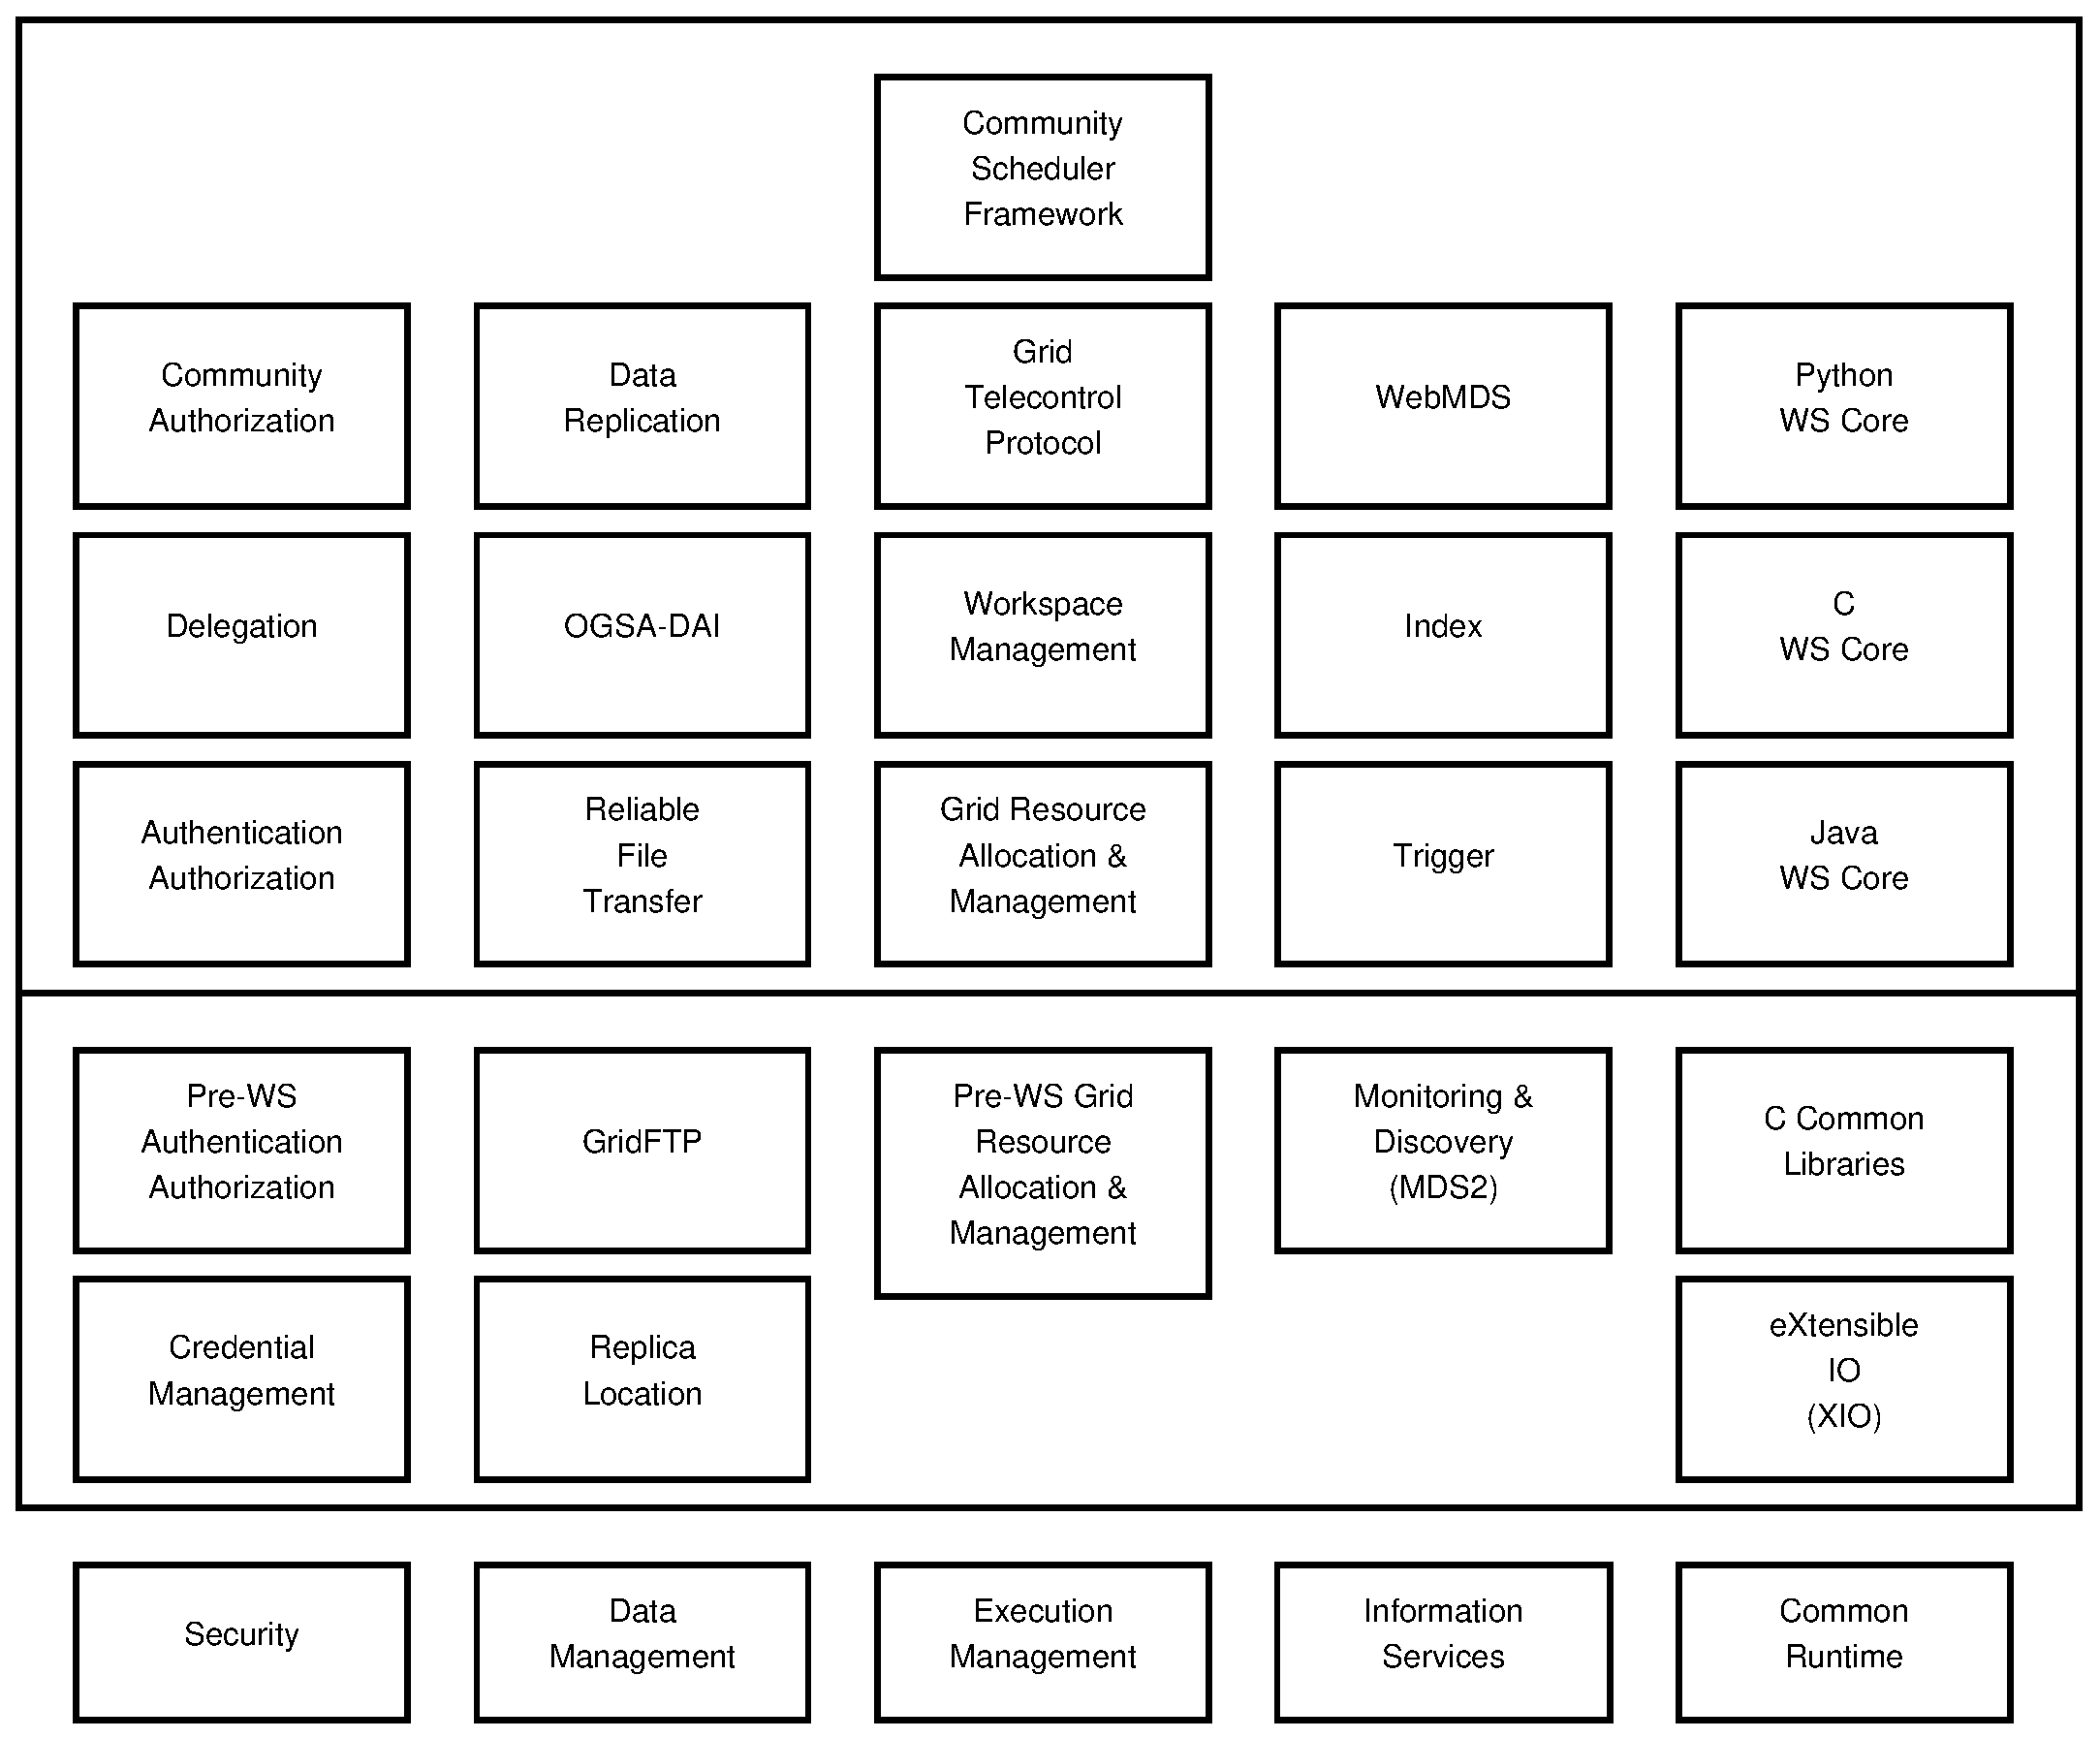
\includegraphics[width=130mm]{images/globus.eps}
\caption{\ac{GT4}}
\label{figure:globus}
\end{figure}

\ac{MDS} is part of Globus Toolkit, and provides the information for the availability and status of grid resources. As a suite of Web Services, it offers a set of components that help to the discovery and monitoring of the resources that are available to a \ac{VO}.

\subsection{gLite}

gLite is a middleware which was created to be used in the operation of the experiment \ac{LHC} in CERN. The user community is grouped in \acp{VO} and the security model is \ac{GSI}. A grid using gLite consists of \ac{UI}, \ac{CE}, \ac{SE}, \ac{WMS} and the Information System.

\begin{figure}[htb]
\centering
 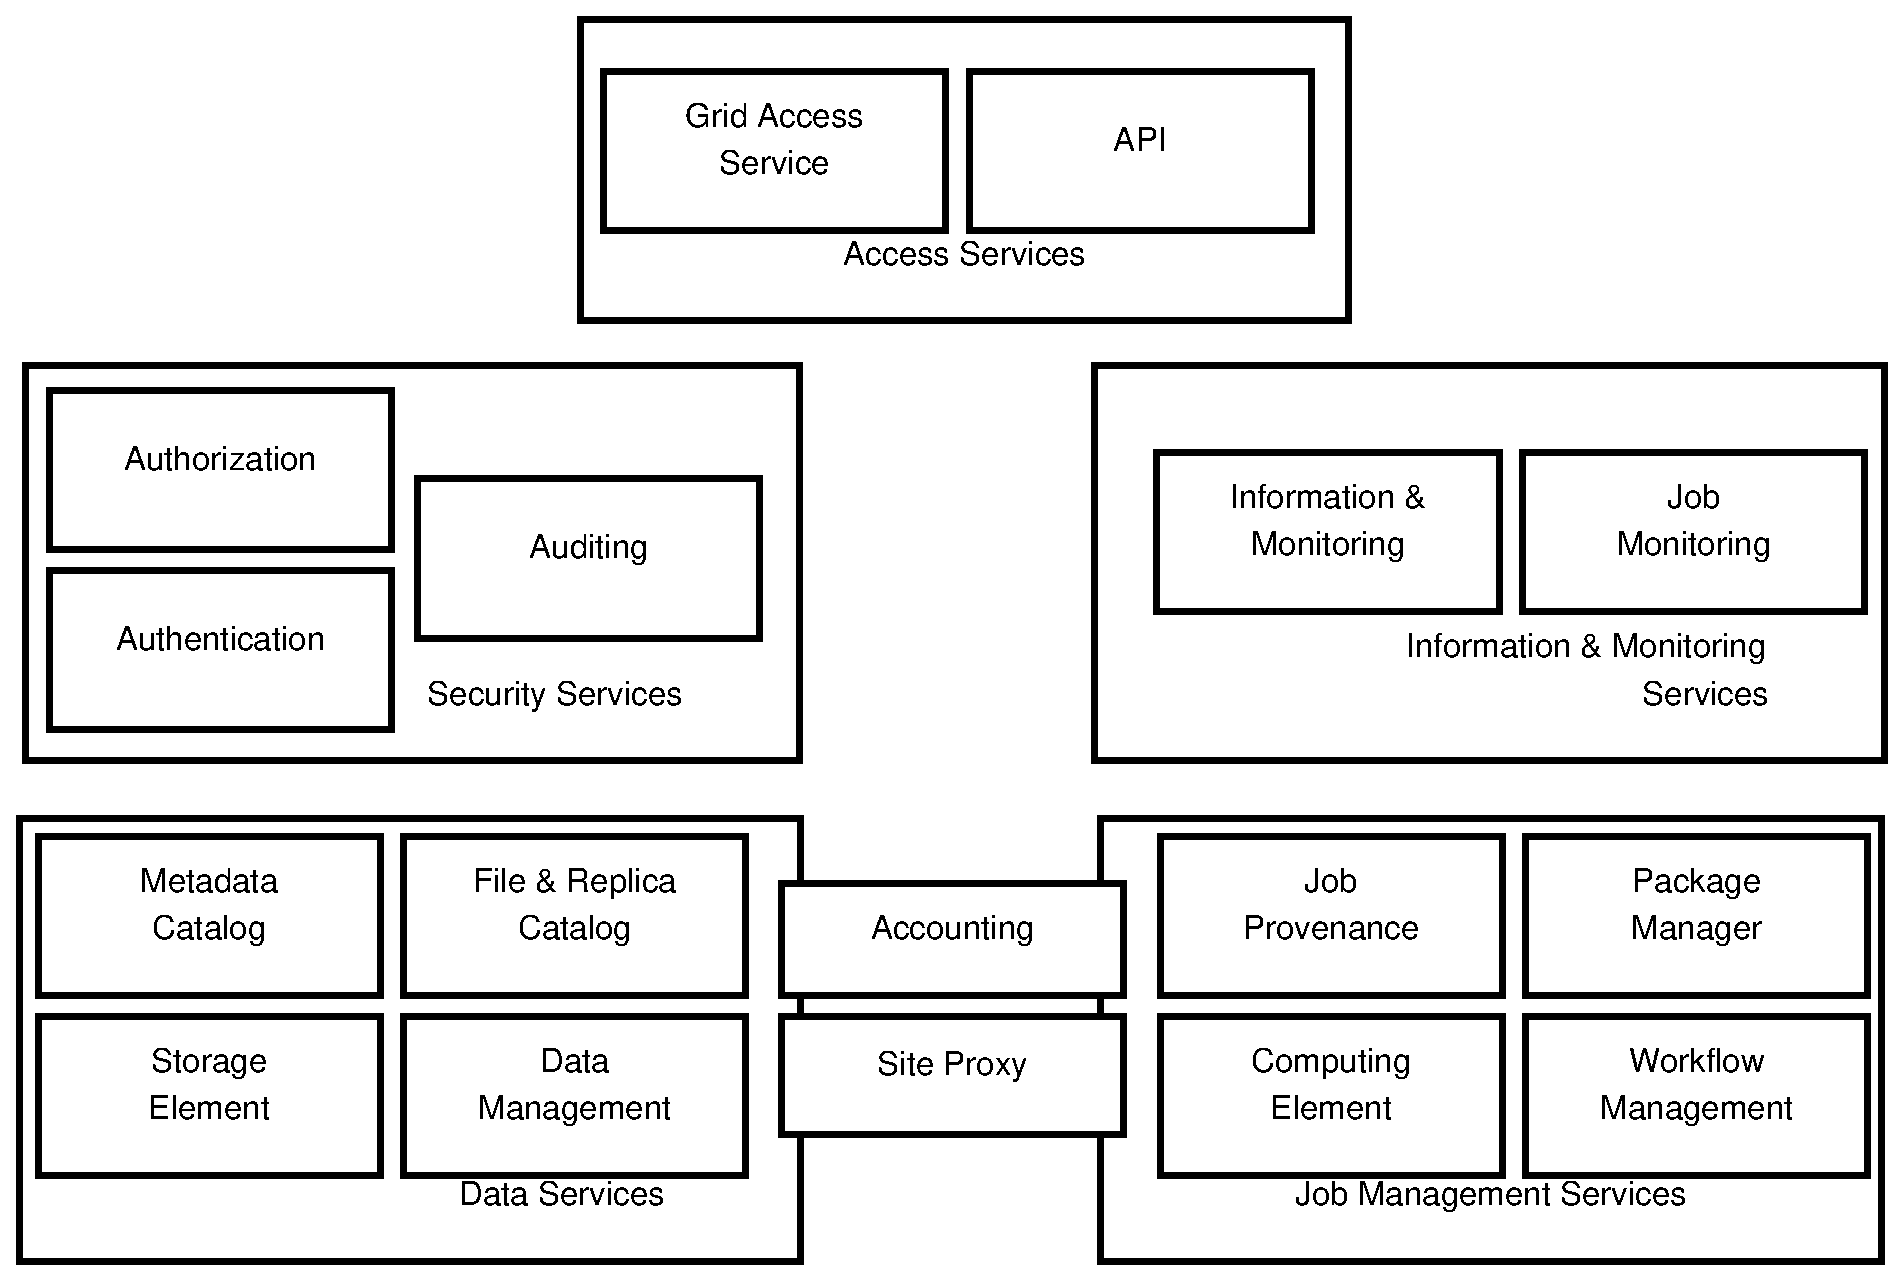
\includegraphics[width=130mm]{images/glite.eps}
\caption{gLite architecture}
\label{figure:glite}
\end{figure}

The information service in version $3.1$ of gLite is almost similar to \ac{MDS} of Globus middleware. The only difference is that the \ac{GRIS} and \ac{GIIS} are provided by \ac{BDII} (see Section \nameref{subsec:BDII}) which is an LDAP based service.

\section{Information Services}
A \ac{GMA} \cite{tierney2002grid} was proposed in early 2000's. Information systems were developed to create repositories of information needed to be stored for monitoring and statistical reporting reasons. Such an organized system later was specified by the \ac{ATP} definition. The largest world grids adopt that model, forming \ac{OIM} in \ac{OSG} (USA) and \ac{GOCDB} as that information base in \ac{EGEE} (Europe). Message Bus was also defined as a mean to transfer the underlying data, and many tools came up such as Gstat, \ac{GOCDB} and \ac{BDII} with Glue specification. Grid performance monitoring and keeping of such an information system has also impact in the performance of the system itself \cite{zhang2003performance}, so various methods were developed to give the solution to the scaling and performance problem, such as \ac{MDS}2 (\ac{GIIS} \& \ac{GRIS}), \ac{GMA} and \ac{R-GMA} \cite{wilson2004information}, which offers relational environment \cite{fisher2001relational}, has experience on production systems \cite{byrom-production} and scales to reach huge needs such as \ac{CMS} project \cite{Bonacorsi2004,Byrom}.

\subsection{\ac{MDS}}
Monitoring and Discovery Services is about collecting, distributing, indexing and archiving information of the status of resources, services and configurations. The collected information is used to detect new services and resources, or to monitor the state of a system.

Globus Toolkit was using LDAP-based implementation for its information system since its early versions, back in 1998 \cite{von1998usage}. \ac{MDS}2 in Globus Toolkit fully implemented referral with a combined \ac{GRIS} and \ac{GIIS}, using mds-vo-name=local to refer to the \ac{GRIS} and all other strings to refer to a \ac{GIIS}. It was widely accepted as a standard implementation of a grid information system \cite{945188}, with good scalability and performance \cite{zhang2004performance}.


\ac{MDS} 4 consists of the \ac{WSRF} and a web service data browser, WebMDS. The \ac{WSRF} Aggregator Framework includes:

\begin{enumerate}
  \item MDS-Index, which provides a collection of services monitoring information and an interface to query such information.
  \item MDS-Trigger, which provides a mechanism to take action on collected information.
  \item MDS-Archive, is planned for future release of MDS, to provide access to archived data of monitoring information.
\end{enumerate}

External software components that are used to collect information (such as Ganglia)\cite{gangliaWSRF} are called Information Providers.


\subsection{Glue}
As long as Information Services are used to connect different infrastructures, the schema of its structure had to be standardized. To interoperate EU and USA grids, DataTAG developed the \ac{GLUE} schema implementation. \ac{GLUE} specification quickly was adopted by the communities and currently its recommended LDAP \ac{DIT} is specified in \ac{GLUE} specification v.$2.0$ from GLUE Working Group of \ac{OSG}.

Many objectclasses of the Glue schema define a \ac{CE}, a \ac{SE}, etc. As seen in Figure \ref{figure:gluece_ext} in later chapter, performance monitoring attributes such as processor load, are defined in objectclasses that extend Computer Element objectclass.

\subsection{BDII}\label{subsec:BDII}
\ac{BDII} is used by gLite as the Information Index Service of the \ac{LHC} experiment. It is LDAP based and may be at top-level or site-level. The \ac{GIIS} has been replaced by site \ac{BDII}, which is fundamental for a site in order to be visible in the grid.

Top-level \ac{BDII} contains aggregated information about the sites and the services they provide. Site \ac{BDII} collects the information from its \acp{CE}, \acp{SE}, etc. It also collects information for each configured service that is installed on the site.

Information about the status of a service and its parameters is pushed on \ac{BDII} using external processes. An information provider is also used (such as in \ac{WSRF}) to describe the service attributes using the \ac{GLUE} schema.

\begin{figure}[htb]
\centering
 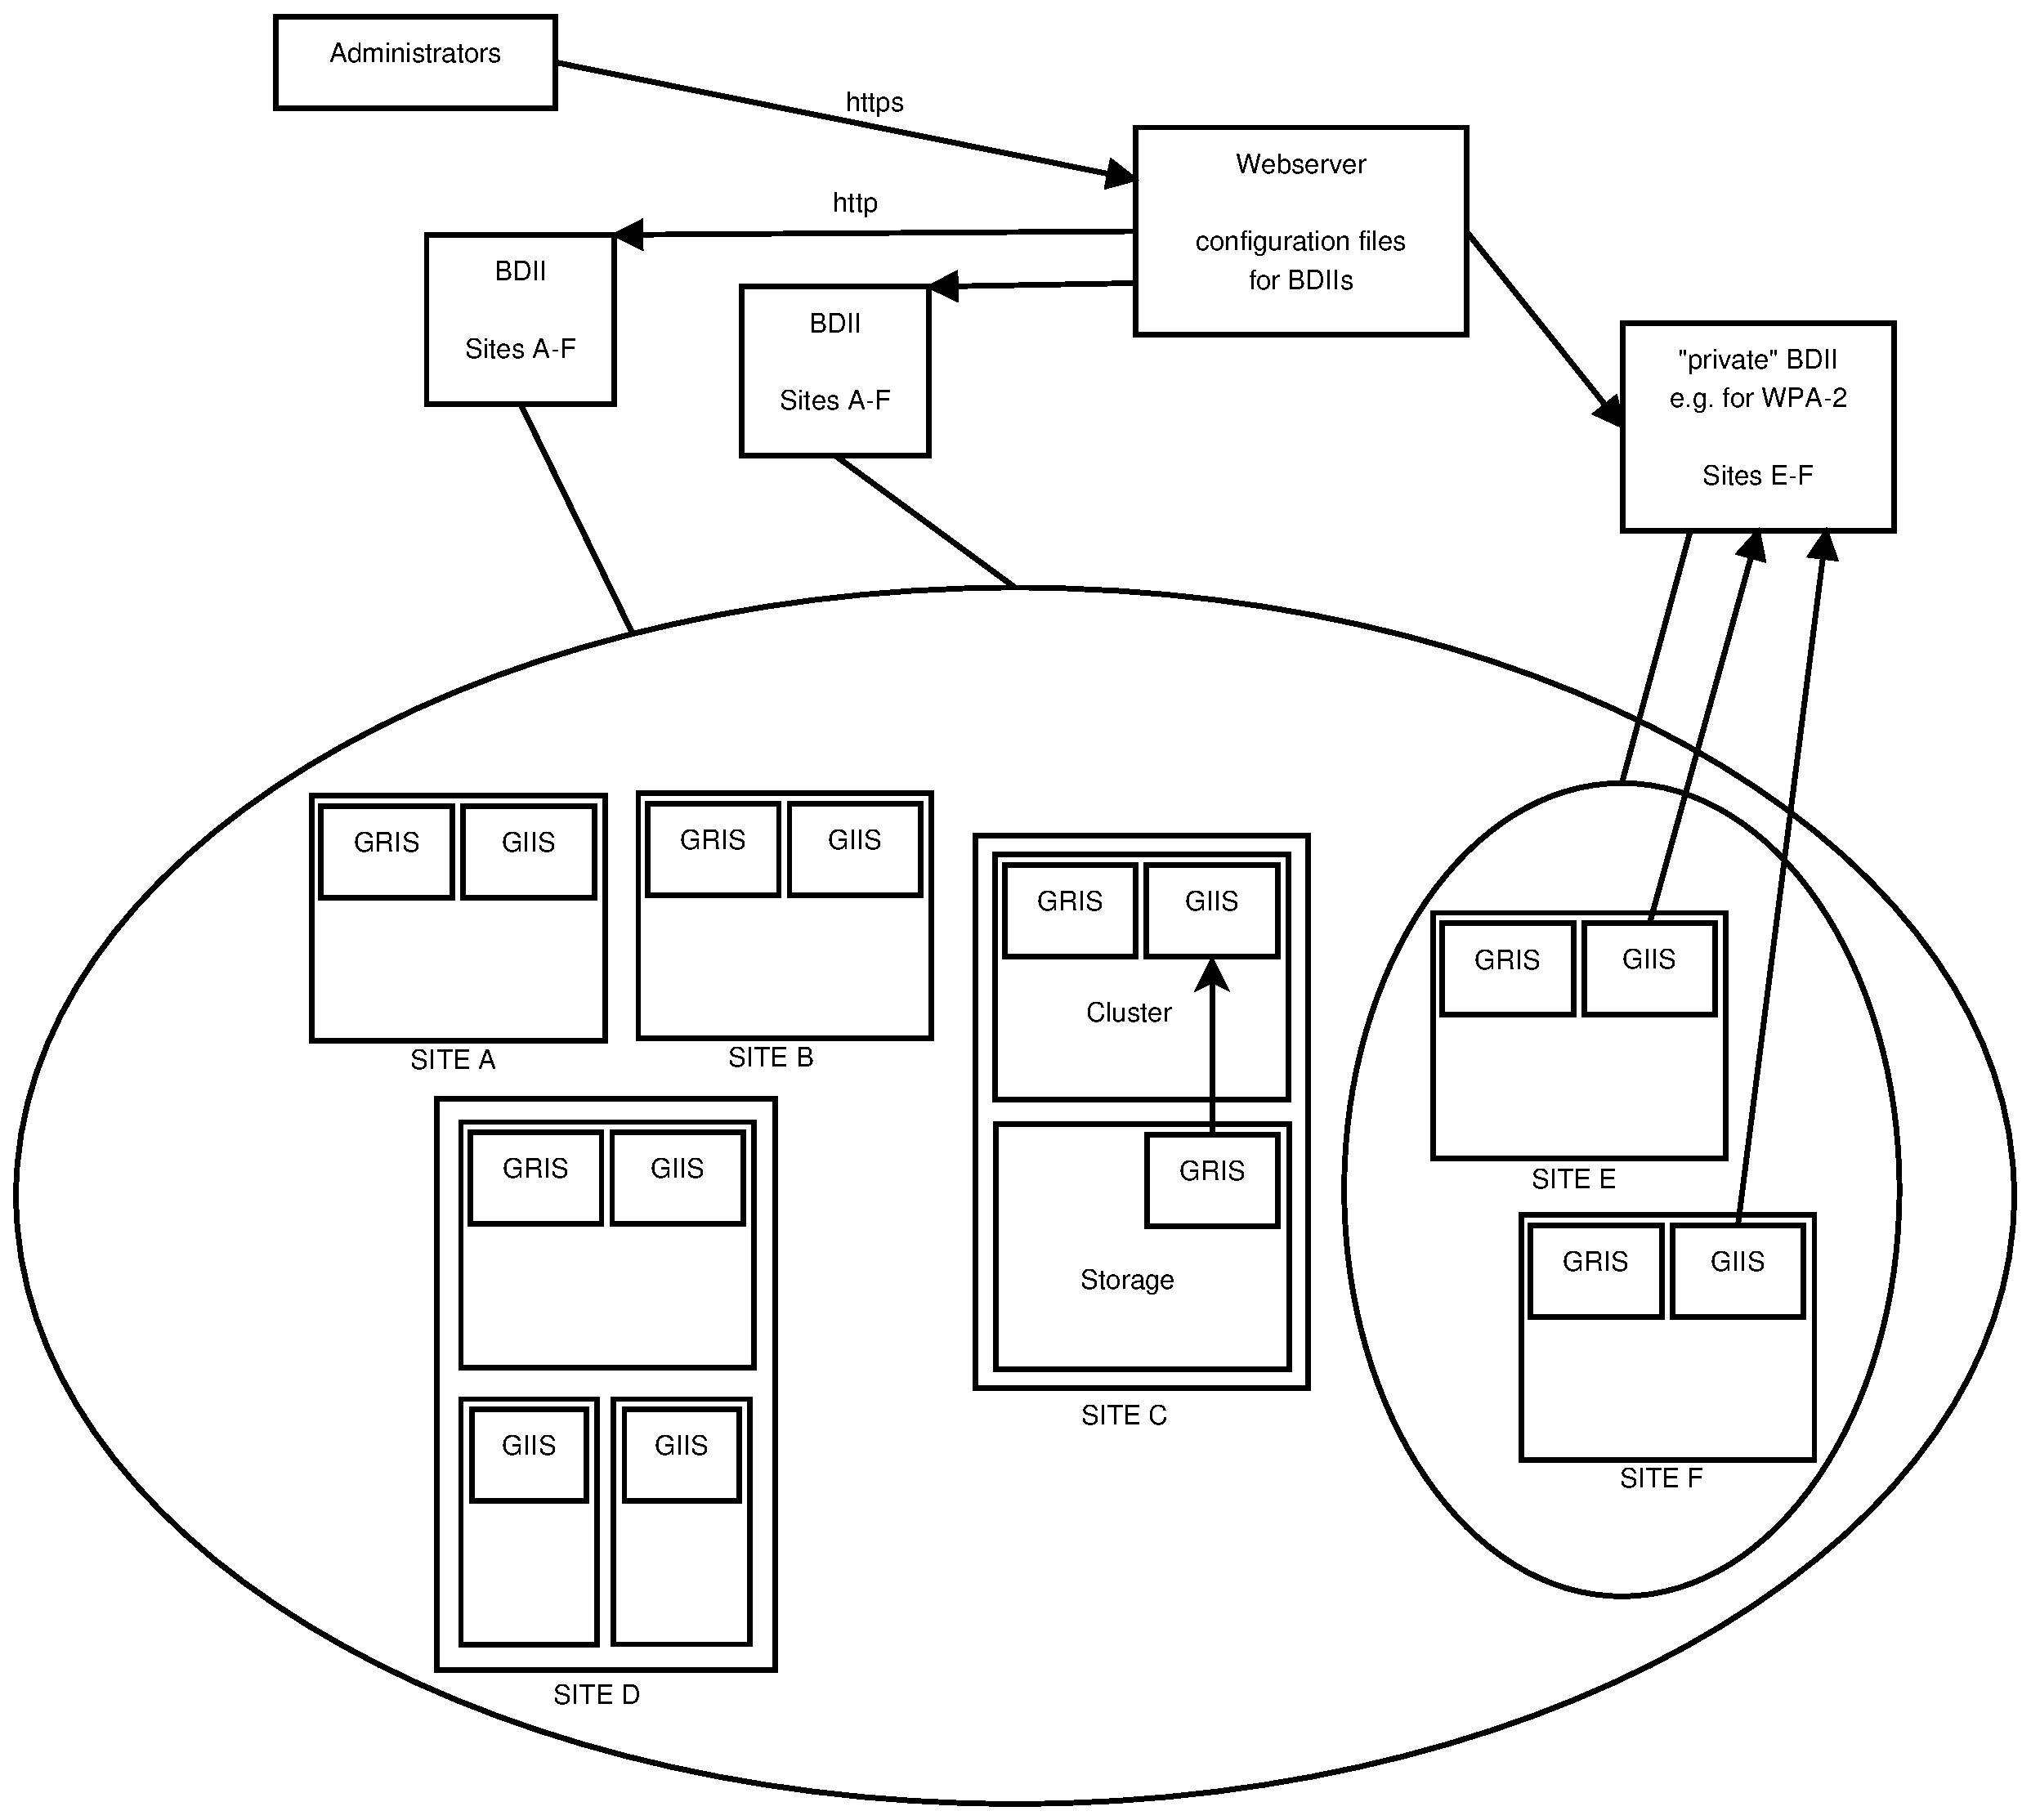
\includegraphics[width=130mm]{images/bdii.eps}
\caption{\ac{BDII}}
\label{figure:bdii}
\end{figure}

\section{Performance Monitoring}
After \ac{EGEE}, the \ac{EGI} was formed to lead in the explosion of the european grid computing community to regional initiatives. Performance and availability monitoring tools and views also follow that format. The result is the phase out of \ac{SAM} \cite{egee3dsa122} and the adoption of Nagios as the tool for regional grid performance monitoring.

A taxonomy effort has been made \cite{gerndt2004performance} to present the differences of performance monitoring systems of the grid, and later a more general \cite{zanikolas2007importance} taxonomy paper was published to give a more general view of these tools. GridICE was generally used to aggregate the performance metrics of \acp{ROC} in high level reports \cite{andreozzi2005gridice}. Later GridICE was left, as \ac{SAM} did, to meet the milestone of \ac{EGI} to have a regional monitoring tool (Nagios) to report the reliability of the joined sites and report the values for \ac{SLA} reasons.

Grid performance can be also measured using benchmark tools in different levels of the grid architecture, using the micro-benchmarks at the Worker Node level, the Site (\ac{CE}) level and the Grid \ac{VO} level. Different metrics and benchmarks exist, such as the measurement of the performance of CPUs in {\bf MIPS using EPWhetstone} and the evaluation of the performance of a CPU in {\bf FLOP/s and MB/s using BlasBench}. GridBench \cite{gridbench} provides a framework to collect those metrics using its own description language, \ac{GBDL}.

GcpSensor \cite{gcpsensor} introduce a new performance metric called WMFLOPS. It uses \ac{PAPI} \cite{papi} to access the hardware performance counters. For data distribution it uses \ac{MDS} information system which provides dynamic metrics for CPU load average for 1, 5 and 15 minutes load.

Linux kernel provides built-in functions to monitor system performance using a metric called $load$. It is a method of individual system performance reporting based on the counter of processes running or waiting in the queue of the Operating System scheduler. This differs from the percentage load average report.

This project focuses on mathematically compute of the performance of a grid based on the metrics that are taken at the Worker Node level.

\subsection{Ganglia}

Ganglia is a monitoring tool which provides a complete real time monitoring environment. It is used by both academia and industry community to monitor large installations of clusters and grids. Any number of host metrics may be monitored in real time using the monitoring core, a multithreaded daemon called Gmond. It runs on every host that is in scope of monitoring. Its four main responsibilities are:

\begin{enumerate}
\item Monitor the changes that happen in the host state
\item Multicast over the network, the changes that has been made
\item Listen to network for changes that other ganglia nodes are multicasting and
\item Answer the status of the whole cluster to specific requests, using XML.
\end{enumerate}

\begin{figure}[ht]
\centering
 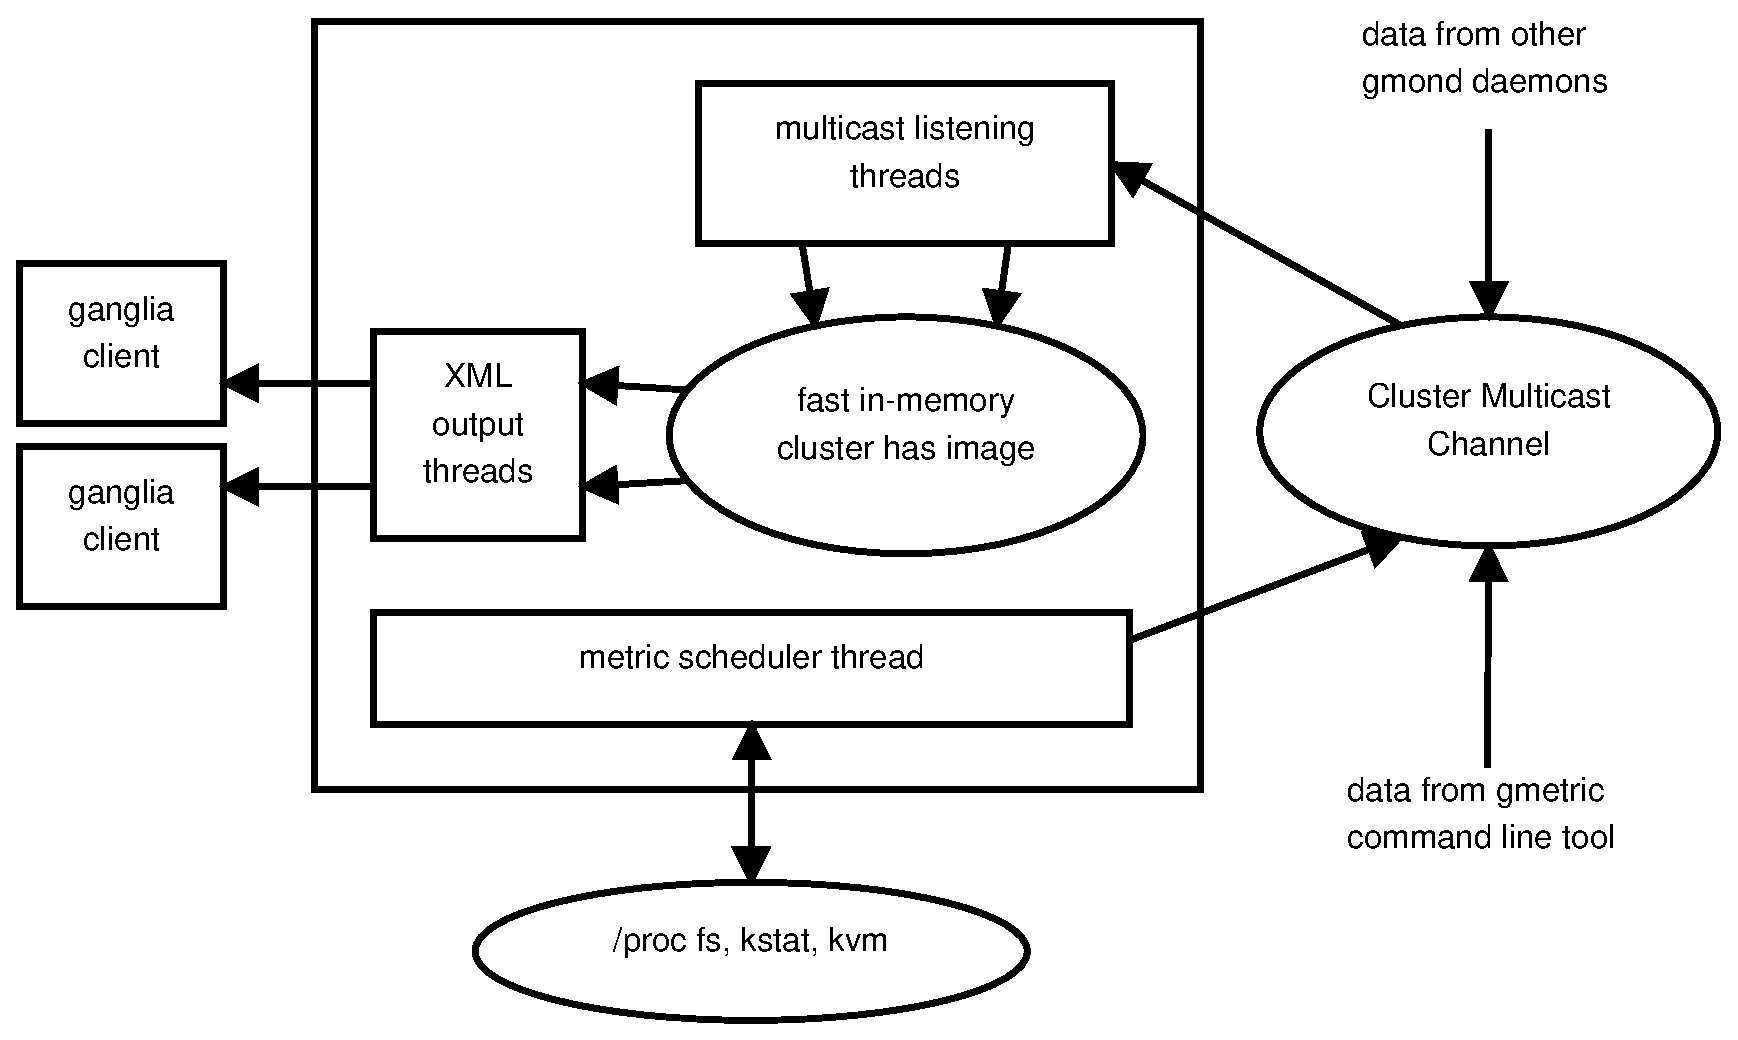
\includegraphics[width=130mm]{images/ganglia.eps}
\caption{Ganglia Data Flow}
\label{figure:ganglia}
\end{figure}

All the data that are gathered from the multicast channel are written to a hash table in memory. The metric data of each node that runs gmond and sends information over the multicast channel are been processed and saved. To send data over the multicast channel, Gmond uses \ac{XDR}. When there is a request over a TCP connection, the response is in XML.

\subsection{Nagios}
Nagios is a monitoring system which provide a scheduler to check hosts and services periodically, and report their status in a \ac{CGI} developed interface. Its large acceptance in industry to monitor service availability has created a large community of developers of custom check commands (plug-ins). It was also accepted from the grid community as the replacement of \ac{SAM} in front of its metrics to periodically parse data from information providers about services availability.

Nagios has a strong back-end, which offers a message bus to integrate with other Nagios installations, to offer the scalability needed to connect site, regional and top level Nagios installations. Information Providers of other Information Services may be customized to be used as Nagios plugins.

Its web based front-end allows the integration with \ac{GOCDB} to handle authentication, using \ac{VOMS} to HTPASSWD system service. Tickets about problems or scheduled downtimes are also handled using Nagios.

Finally, its backend may be scaled-out by using NDOUtils as a service to offer database for the logging of check operations and history. PNP4Nagios is a plug-in that offers visualization of the performance metrics, using the RRDTool. Its distributed monitoring solutions recently were expanded by the \ac{DNX} and the \ac{MNTOS} \cite{Nagios}

\section{European Grid Infrastructure}
Latest \ac{EGI} directive to form regional operation tools forced the use of Nagios \cite{imamagic2007grid} as the main tool of availability \& performance (an so reliability) monitoring of the grid. Each \ac{NGI}/\ac{ROC} (regional level) has its own interface, and hierarchically there is a Super Nagios interface to report the top level view of general system availability. Nagios offers extensions such as NRPE to remotely invoke check commands in inaccessible/private installations. Another important add-on to Nagios is the NdoUtils, which offers an SQL store of history data to the monitoring interface. Nagios Configuration Generator was introduced to help the automatically generation of the configuration based on the information system of nodes and services.

Finally, there has been proposed an integration of \ac{SAM} views to a Nagios customized interface, to offer the last good known \ac{SAM} interface to the old users. Nagios also integrates with \ac{GGUS}, a ticketing system that european grid initiative uses. Monitoring infrastructure in EGI is fully distributed using regional Nagios servers and the corresponding regional MyEGI portals.

\subsection{UK Initiatives}
Brunel University takes part in regional and european initiatives. 5 different \acp{CE} exist, and 3 \acp{SE}, consisting the UKI-LT2-Brunel site. LT2 stands for London Grid, a co-operation with other London Universities. \ac{GridPP} and \ac{NGS} are two collaboration groups that Brunel University is member of.

In \ac{GridPP}, regional monitoring tools exist to provide distributed monitoring services in UK. Regional Nagios and MyEGI/MyEGEE instances co-exist in Oxford University that offer service availability monitoring for all UK sites. Ganglia installations exist in site level deployments, and a Ganglia frontend which aggregates Tier-1 sites is offered through \ac{RAL}.

\chapter{Design/Methods}
\section{Approach Adopted}
\section{Design Methods}
\section{Data-acquisition Systems}
\section{Range of cases ecamined}
\chapter{Results}
% chapter Results

\section{Events source}

Results are examined on the generation of metrics, during the aggregation using various information services and they are presented using ready and custom developed interfaces.

\subsection{Unix stuff}

As described in subsection \nameref{subsec:metrics} of the previous chapter, Linux provides through the {\bf proc pseudo-filesystem} a simple file interface to the metrics taken from the scheduler of processes that are queued in the processor.

The three metrics about CPU load on 1, 5 and 15 minutes average are displayed as follow:

\begin{verbatim}
[root@gr03 ~]# cat /proc/loadavg 
2.29 0.73 0.32 1/230 3584
\end{verbatim}

which may also be displayed using the {\bf uptime command}:

\begin{lstlisting}
[root@gr03 ~]# uptime
 00:01:20 up  1:41,  3 users, load average: 2.29, 0.73, 0.32
\end{lstlisting}

When we examine the Linux kernel source code, there is a macro command named $CALC_LOAD$ which takes the options that have been discussed and returns the result of the metric. The definition of the macro can be seen in file {\bf include/linux/sched.h}, Listing \ref{kernel}.

\subsection{Ganglia}

When gmond starts, it listens on port 8649/TCP by default, to accept TCP connections and throw XML report for the whole cluster. It also binds to the multicast address on port 8649/UDP to get other hosts messages for metrics changes, and also multicast its own metrics. Listing \ref{lsof} shows the opened sockets of Gmond daemon, and Listing \ref{telnet_gmond} display a sample xml output when connecting to 8649/TCP to transfer metrics through XML.

Worker nodes are configured to transfer metrics data using multicast. Each Gmond daemon of each Computing Element node, by Ganglia definition has to know the state of the whole Computing Element cluster. Using standard UNIX commands to listen to the data transferred on the multicast network, a sample transfer of load\_one metric is observed (Listing \ref{tcpdump}). As described in Subsection \ref{subsec:ganglia}, metric data are multicasted by Gmond when there is a change in the value, or when the time threshold is reached.

Using Ganglia build-in command $gstat$, a nice output of Processor Load metrics is shown for the whole cluster in Listing \ref{gstat}

\begin{lstlisting}[language=bash,caption=Gstat output,label=gstat]
[root@gr01 ~]# gstat -al1
gr03.oslab.teipir.gr     2 (    0/   87) [  0.00,  0.00,  0.00] [   0.0,   0.0,   0.0,  99.9,   0.1] OFF
gr01.oslab.teipir.gr     1 (    0/   75) [  0.00,  0.00,  0.00] [   0.0,   0.0,   0.0,  99.9,   0.0] OFF
gr02.oslab.teipir.gr     1 (    0/   99) [  0.00,  0.00,  0.00] [   0.0,   0.0,   0.1,  99.9,   0.0] OFF
\end{lstlisting}

\section{Aggregation and transfer}

Metrics taken from the event source are passed to the information service using the information/resource provider.

\subsection{WSRF}

In WSRF the $wsrf-query$ command is executed using the URL of the container where the WSRF was been deployed. The container should run in a host with a host certificate signed by a certificate authority, and a certificate proxy should be initialized with a valid user certificate that is requesting the information. 

\begin{lstlisting}
/opt/globus/bin/wsrf-query -s https://osweb.teipir.gr:8443/wsrf/services/DefaultIndexService "//*[local-name()='Host']"
\end{lstlisting}

The result of the above query returns a list of all cluster nodes. An abstract result is displayed here in Listing \ref{wsrfquery}.

\subsubsection{WebMDS and XPath}

The role-based access control model of the grid security context allow queries only by authenticated and authorized users. Building a testbed with full grid security in mind would be out of this project scope, so XML result of Web Service calls is taken through WebMDS instead of \ac{WSDL} discovery and \ac{SOAP} messaging.

Using the following XPath query in the WebMDS form, a request to get the metrics of Host node with name $ltsp.oslab.teipir.gr$ was sent.

\begin{verbatim}
//glue:Host[@glue:Name='ltsp.oslab.teipir.gr']
\end{verbatim}

WebMDS match the query in its cache and replies only the specific node that was requested. If the cache was expired (its default value is 60 seconds) the information system uses the Resource Provider to fetch the XML from Gmond and transform it using XSLT to Glue schema and serve the new values as shown in Listing \ref{xpath_result}.

\subsection{BDII}

On the other information service, using $ldapsearch$ command and specifying the base DN for the search, the host URI and the desired attributes to return, we may get the values asked from the BDII as seen on Listing \ref{ldapsearchbdii}.

\begin{lstlisting}[language=bash,caption=BDII LDAP search for Glue CE ProcessorLoad attributes,label=ldapsearchbdii]
# ldapsearch -H ldap://osweb.teipir.gr:2170 -x \
-b GlueHostName=ainex.local,Mds-Vo-name=local,o=grid \
GlueHostProcessorLoadLast1Min GlueHostProcessorLoadLast5Min \
GlueHostProcessorLoadLast15Min

# ainex.local, local, grid
dn: GlueHostName=ainex.local,Mds-Vo-name=local,o=grid
GlueHostProcessorLoadLast1Min: 27
GlueHostProcessorLoadLast15Min: 22
GlueHostProcessorLoadLast5Min: 20
\end{lstlisting}

The above information has been given by the BDII LDAP instance which used the wrapper of Ganglia Resource Provider, a customized Perl script to export MDS format as shown in Listing \ref{perlbdii}.

Using the Ganglia official python client (Listing \ref{pythonbdii}) which is distributed with the source code of Ganglia Client, rejected as an option because Perl is easier in handling regular expressions for string operations and transformation.

\section{Presentation}

Finally, to present the information, two custom interfaces have been developed in PHP. Both programs reside in Brunel University webserver which supports the needed libraries and network connections. The source code is available under that page, and when called using BDII or WSRF, the result is exactly the same and looks like Table \ref{tab:html_output}.

\begin{table}[ht]
\centering
%\small\addtolength{\tabcolsep}{-3pt}
\begin{tabular}{ | l | l | l | l | l |}
\hline
 Hostname & 1min & 5min & 15min \\ \hline
 ltsp.oslab.teipir.gr & \colorbox{green}{0.01} & \colorbox{green}{0.09} & \colorbox{green}{0.09} \\ \hline
 xenia.oslab.teipir.gr & \colorbox{green}{0.00} & \colorbox{green}{0.06} & \colorbox{green}{0.06} \\ \hline
 gr201.oslab.teipir.gr & \colorbox{green}{0.52} & \colorbox{green}{0.59} & \colorbox{green}{0.42} \\ \hline
 gr130.oslab.teipir.gr & \colorbox{green}{0.00} & \colorbox{green}{0.06} & \colorbox{green}{0.16} \\ \hline
 gr131.oslab.teipir.gr & \colorbox{yellow}{1.22} & \colorbox{green}{0.79} & \colorbox{green}{0.40} \\ \hline
 gr212.oslab.teipir.gr & \colorbox{green}{0.06} & \colorbox{green}{0.09} & \colorbox{green}{0.09} \\ \hline
 gr180.oslab.teipir.gr & \colorbox{red}{2.06} & \colorbox{yellow}{1.49} & \colorbox{green}{0.59} \\ \hline
 gr181.oslab.teipir.gr & \colorbox{green}{0.71} & \colorbox{green}{0.57} & \colorbox{green}{0.32} \\ \hline
\end{tabular}
\caption{Sample output from both calls with DOM or LDAP}
\label{tab:html_output}
\end{table}

Page \url{http://people.brunel.ac.uk/~dc09ttp} contains complete results using both DOM and LDAP methods.

\subsection{DOM}

The first interface uses PHP \ac{DOM} functions to call the WebMDS and get the XML as it would happened by calling the WSRF Web Service with native SOAP messages and authentication. Listing \ref{wsrf.php} is an abstraction of the code deployed in Brunel's webserver and returns only one value. The purpose of this listing is to present the use of functions and not the HTML stuff.

\begin{lstlisting}[language=PHP,caption=PHP DOM call to WebMDS,label=wsrf.php]
$url="http://osweb.teipir.gr:8080/webmds/webmds?info=indexinfo&xsl=&xmlSource.indexinfo.param.xpathQuery=%2F%2F*[local-name%28%29%3D%27Host%27]";
$file  = file_get_contents($url);
$dom = DOMDocument::loadXML($file);
$host = $dom->getElementsByTagName('Host');
$procload = $host->item($k)->getElementsByTagName('ProcessorLoad');
echo ($procload->item($i)->getAttribute('Last1Min'))/100;
\end{lstlisting}

\subsection{LDAP}

The second interface uses LDAP functions to connect to BDII instance and get the results from objects that instantiates the GlueHostProcessorLoad class. Listing \ref{bdii.php} displays the method to bind anonymously, form the query and get a sample result.

\begin{lstlisting}[language=PHP,caption=PHP LDAP call to BDII,label=bdii.php]
$ds=ldap_connect("osweb.teipir.gr","2170");
if ($ds)
{
    $r=ldap_bind($ds);
    $sr=ldap_search($ds, "mds-vo-name=local,o=grid", "(&(objectClass=GlueHostProcessorLoad))");
    if ($sr)
    {
         $info = ldap_get_entries($ds, $sr) or die("could not fetch entries");
         echo ($info[0][gluehostprocessorloadlast1min][0])/100;
    }
ldap_close($ds);
}
\end{lstlisting}

\subsection{Nagios}

Nagios calls check\_ganglia periodically (configured as check interval) and logs the state of each service and host check. Load averages are described as services. Listing \ref{nagioslog} shows the log file of nagios service check for these values straight from Ganglia.

\ac{NPCD} is configured in bulk mode so a file may be found in the spool directory before the interval passes to process it with perl script to \ac{RRD} database. Listing \ref{npcdfile} contains the performance data metrics.

Finally, Nagios Web interface displays the aggregated values of host performance state in multiple views, as shown in Table \ref{tab:nagios_service_detail}.

\begin{table}[ht]
\small\addtolength{\tabcolsep}{-3pt}
\scalebox{0.8}{
\begin{tabular}{ | l | l | l | l | l |}
\hline
 Host & Service & Status & Last Check & Status Information \\ \hline
 gr129 & load\_fifteen & \colorbox{green}{OK} & 02-08-2011 20:17:23 & CHECKGANGLIA OK: load\_fifteen is 0.17 \\
\hline
  & load\_five & \colorbox{green}{OK} & 02-08-2011 20:18:12 & CHECKGANGLIA OK: load\_five is 0.27 \\
\hline
  & load\_one & \colorbox{green}{OK} & 02-08-2011 20:17:43 & CHECKGANGLIA OK: load\_one is 0.02 \\
\hline
 gr130 & load\_fifteen & \colorbox{green}{OK} & 02-08-2011 20:14:23 & CHECKGANGLIA OK: load\_fifteen is 1.77 \\
\hline
  & load\_five & \colorbox{yellow}{WARNING} & 02-08-2011 20:14:15 & CHECKGANGLIA OK: load\_five is 4.75 \\
\hline
 & load\_one & \colorbox{red}{CRITICAL} & 02-08-2011 20:14:43 & CHECKGANGLIA OK: load\_one is 11.60 \\
\hline
\end{tabular}}
\caption{Example Nagios service status details for ganglia check}
\label{tab:nagios_service_detail}
\end{table}


\chapter{Analysis}
% chapter analysis
\section{Methods Adopted}

In complex distributed systems such as grids, performance bottlenecks may be located using monitoring data. From the processor usage on a single node of a computing element to the total usage of processed jobs in a large cluster, performance data help to focus on the problem that impacts the overall performance.

In order to succeed in grid monitoring, some requirements should be considered. A very large amount of data should be delivered real-time, from many heterogeneous sources on different networks or even countries. These data must be accurate and consistent. There should be synchronized timestamps on the generation of each metric, to the measurement value that should be comparable between different architectures. Hosts time synchronization is achieved with network time protocol, so all metrics are taken on the time that they actually report. Metrics should have error bounds to preserve accuracy, and the consistency issue is solved using coordination of that activity, so the impact of a metric to other sensors is controlled.

The flow of the monitoring process initialization is described from the GMA standard. The application-consumer queries the directory service in order to declare its interest to get metrics for a specific host/cluster. The sensors of the elements that is equivalent to the specific query generates the metrics that will be given to the consumer from the producer, which in turn queries the directory service to find the consumer. The producer is the one that initializes the connection to the consumer in order to deliver the measurements, even if the consumer had asked the directory service for this. \cite{balatonuse}

\subsection{Performance Metrics}

Linux kernel process scheduler provides the three numbers for the processor load during the last one, five and fifteen minutes period. There are many ways to calculate the system load in UNIX systems, updating the values on each scheduler event or periodically sampling the scheduler state.

Scheduler efficiency impact on total system's performance, and periodic sampling lead to more accurate load averages. Linux uses the second one, with the period of five seconds, five clock ticks. Each "clock tick" is represented by the HZ variable which is the pulse rate of a kernel activity. This method is more performance-wise from the first one where recalculation of load occurs in every scheduler event. 

There is a significant difference between processor load and processor usage of a system. Processor usage is a percent representation of the use of CPU by processes, and not used in this project. CPU load is a better metric for the system performance because it does not have a top value of 100\% but is based in processes running and waiting in the scheduler queue.

\subsubsection{Transport and sample}
Gmond code uses the ganglia libmetrics library which in case of Linux operating system parses the $/proc/loadavg$ pseudo-file to get Linux kernel calculated system load average as shown in Listing \ref{libmetrics}. When this value is taken, it is pushed to the multicast network using UDP datagram. If this value has not changed from the previous one, it is not pushed until a timeout is reached.

\subsection{Information Systems}

\subsubsection{WSRF}

The XML that Ganglia Resource Provider took from Gmond process through TCP, is transformed on WSRF using XSLT technology, to another XML document that follows the Glue-CE schema.

Directory $globus\_wsrf\_mds\_usefulrp$ of globus configuration root, includes the file $ganglia\_to\_glue.xslt$, where we can focus on the transformation rules. A snippet of interest for the case of ProcessorLoad class is seen in Listing \ref{xslt}. There, XPath queries are visible and a multiplication with 100 on CPU load values to get an integer is executed. This is happening in order to avoid the transfer of float values. In the frontend using DOM, a division with 100 is done to get the original CPU load average number back.

\subsubsection{BDII}

On the other hand, in BDII Processor Load values left as decimal numbers because its easy for LDAP to handle string values of numbers. The transformation from Gmond or Gmetad information provided using XML, is done by Perl $XML::Parse$ and the output is given in MDS format. There were also some changes performed to the original Perl script, written by Stratos Efstathiadis, to match testbed's LDAP schema \cite{stratos_efstathiadis}.

\subsection{Nagios}

Nagios was installed in the testbed using \ac{YAIM} tool. Some user certificates from \ac{TEIPIR} and Brunel was added to access the interface through the VOMS2HTPASSWD tool.

Custom check command was introduced to configure Nagios with ganglia. Ganglia original check\_ganglia.py client was used as shown in Listing \ref{checkganglia}.

Nagios service check templates were created, to match all nodes of hostgroup named $worker-nodes$, one for each of the three metrics that will be aggregated in Nagios. Under the configuration listed in Listing \ref{nagiosservice}, options for warning and critical thresholds of Processor Load applied, to notify the contacts that will be set to monitor these services through the rest of Nagios system.

\section{Grid Performance and Site Reliability}

Grid monitoring in general as proposed by Multi-Level Monitoring in EGEE Service Activity SA1, is about availability and reliability monitoring. There are threshold values for these metrics for a production site and SLA calculation make use of these metrics.

The main purpose of performance monitoring, when examined from this point of view, is to count jobs that are successfully being submitted to a \ac{CE}. Site reliability is calculated using that metric.

For a system engineer, performance monitoring for system administration has to do with Processor Load metrics and not with jobs failed or executed successfully. With that in mind, a system engineer may take capacity management decisions to scale-out the Computing Element, or even scale-up a single node of it.

This is the main goal of this project, to provide tools that allow the aggregation of Processor Load information to system engineers, and not job counting tools such as \ac{SAM}, Gridview and MyEGEE or MyEGI. Ganglia is the event source that publish the metrics taken from Linux kernel as described, and multiple information services or even Nagios may be used to provide that information to users.

\section{Information Services Scaling}

\subsection{LDAP}

LDAP as the core technology of MDS2 has been investigated \cite{zhang2004performance} and proved that scales and performs good when the data are kept in cache. The performance of the information system, when it is accessed by a large number of concurrent users, degrades dramatically if data caching is not used.

Compared with WSRF, it {\bf performs faster} \cite{schopf2006monitoring} in small number of users, because of the LDAP base of this information service. LDAP back-end is a Berkeley DB and is implemented in C, versus Java and SOAP over HTTP and XML of WSRF. Caching in LDAP although is reported to have problems.

\subsection{WSRF}

On the other side, MDS4 (WSRF) scales better than MDS2 (LDAP) in {\bf large number} of concurrent users. Both throughput and response in queries in large number of queries are consistent, which allows the use of MDS4 for robust operations.

WSRF also supports {\bf many query languages}, unlike BDII which supports only LDAP queries. By default it is distributed only with support of XPath queries, but its architecture which is based in Java container and SOAP/XML standards, allow the distribution of the Information Service with other query languages as well.

Adding a Resource Provider in WSRF was much easier than adding an Information Provider in BDII, which makes MDS4 more {\bf extensible} than MDS2. Even though in BDII a simple wrapper had to be installed in BDII \ac{GIP} configuration directory, the Perl script (or the Python one provider by Ganglia) had to be changed to reach the running BDII instance of Glue schema. MDS4 and WSRF are based in XML and XSLT transformation mechanisms that allow the easy addition of other Providers of a site. It is even allowed to aggregate Index Services from other sites using the $downstream$ option to register them in the local Index Service.

BDII LDAP based configuration is complex due to OID namespaces and naming authorities and is not portable with other information systems. WSRF configuration is much easier and {\bf flexible} because of the XML-based information model, which generally is considered more friendly.

{\bf Reliability} is another factor where WSRF is better than LDAP. BDII after a long period of heavy activity has memory usage problems and requests may have delay in being served, so periodically service restarts are needed, unlike WSRF Index which has been tested under heavy load and keeps serving without problems \cite{schopf2006monitoring}.

Although WSRF in many factors is dominating, during this project some problems occured when some nodes of the Computing Element are down. Some deserialization exceptions appear in the container log file for a few minutes until the WSRF learn about the new state of the cluster from Gmond.

\chapter{Conclusions}
% chapter Conclusions

Grid monitoring is an important factor when working with Grid Systems. Reports extracted from monitoring systems, support decisions for capacity management, and prove that a system meets requirements needed for Service Level Agreements.

Metrics for Computing Element performance monitoring usually are:

\begin{enumerate}
 \item {\bf Total Jobs} in running or waiting to run state.
 \item Individual per working node {\bf Processor Load}.
 \item {\bf Benchmarking} metrics such as FLOP/s.
\end{enumerate}

This project focused in the calculation, aggregation and transfer to present the metrics for Processor Load of working nodes of a Computing Element. Running and waiting jobs monitoring is extremely analyzed under availability monitoring research.

Calculation using the number of processes waiting in the queue of kernel scheduler where used. This metric is explained why is more accurate from the classic percentage CPU usage.

Aggregation and transfer of metrics where examined in many different levels, from the multicasted XDR of Gmond to the resource providers of the information service that where used.

Information Service is core technology that used in Grid Computing. It has evolved in parallel with Middleware. Current version of the Monitoring and Discovery Service standard has reached the MDS4, introducing the use of Web Services. MDS2 was based in LDAP, which is still used by some systems to discover services.

Nagios bulk aggregation features using NPCD and MSG-Nagios-Bridge also provide a method to aggregate Ganglia metrics without the use of the MDS.

Presentation where simply examined using:

\begin{enumerate}
 \item {\bf DOM technology} to parse XML taken from WSRF through WebMDS interface using XPath
 \item simple {\bf LDAP} communication to take the metrics from the BDII Information Service
\end{enumerate}

\section{Conclusions}

Every aspect of grid monitoring keeps {\bf scalability in mind}. Distribution of metrics in all worker nodes using Gmond is the key to keep redundant that information.

BDII Information Service is great for use in site level environment, as LDAP performs faster than WSRF in less than a hundred users.

Site monitoring needs Nagios and Ganglia for a few hundreds of nodes. Nagios web interface is enough for site-level host and service view. Ganglia web interface supports good aggregation of many clusters, to the Region-level.

WSRF caching feature, Indexer and Aggregator Framework scales better and may be used for regional and top level monitoring.

Heterogeneous environments should {\bf rely on standards} in order to inter-operate and stay reliable. Even the Information Services mentioned above stick to the Glue schema.

A tool may seem to be great for its purpose, but after focusing on a need is may be discontinued, such as SAM. This example is taken from the availability monitoring as its frontend were replaced by MyEGI and Nagios keeping its back-end in MRS.

\section{Further Work}

\subsection{Aggregation}

Additional investigation is required to be carried out for the aggregation of collected information. WSRF offer the Aggregator Framework, which downstream information from many EPRs and deliver it through the Index service. To scale such information in the Regional monitoring level may have issues that only in that scale will came out.

\subsection{Benchmarking}

Performance metrics which are produced using benchmarking software is good standard way of measuring and advertise the performance of Computing Elements. Such metrics are not efficient for regularly runs and frequently changes because they are cost effective performance wise. It is good although to present the performance ability of a CE, so if they could be executed every some long time periods and pushed in the information service, will offer a good metric to select one CE of another.

\subsection{Storage element performance monitoring}

Storage Element performance monitoring is an interesting area for research. Vendors that produce enterprise level storage systems also offer tools to monitor the performance of the storage system. Most used metric is I/O Operations per second and throughput in GByte per second, in every aspect of a storage system.

Storage systems are also provided by different vendors and may also deployed as custom solution. Fiber Channel solutions versus Clustered File System cases are examined \cite{brzezniak2008analysis} as a chapter of distributed systems, storage oriented.

Hadoop is the most commonly used distributed data storage. In CMS, an experiment that is known for its huge needs in data storage, Hadoop has been adopted \cite{hadoop} as the distributed file system. Grid computing community have adopted the use of Total and Used GB per Storage Element (as in Computing Element), but there is still enough work on the performance monitoring.


\backmatter

\bibliographystyle{ieeetr}
\nocite{*}
\bibliography{extra/books}

%\label{appb}
%\lhead{Appendix B. \emph{Interim Report}}
%\section{Introduction}

In EGI era of grid computing in Europe, MyEGEE and Nagios are taking the place of SAM in performance monitoring of the grid, in NGI oriented infrastructures. SAM Framework had a significant role in reporting the service availability. That monitoring model was needed to be replaced by a new Multi Level Monitoring architecture. The need of establishing a central point in regional level, where metrics gathered from each information system of the grid, lead to the adoption of MyOSG. MyEGEE is the tool that extends MyOSG to European NGI's and provides an interface to customize the display of aggregated metrics of the performance of NGI sites. Nagios is the main technological choice to provide that regional monitoring system.

\section{Aims and Objectives}

Different role users are going to use a portal to get information about the performance status of the grid, to export the appropriate report for their job. This project aims to develop these particular pieces of code to support the aggregation of the metrics from Nagios, to allow the web based customization of the visualization of the reports. These metrics are needed to report the availability and reliability of NGIs and particular sites of the grid.

The procedures that are going to be used in order to achieve the above aims should include at the beginning some opening and exploration of the environment where the interface is going to be placed. The usage of grid computing in the world should be well known, so a visibility of the importance and the possible uses of the software will be recognized. The appropriate access to the infrastructure should be gained, on different platforms and levels. Brunel University site and GridPP/NGS VO at the beginning, as long as the UKI ROC operations may be a good point of collaboration with researchers to reach the bests possible requirements and data to analyze. The middleware used in both these VOs should be examined so with the knowledge of running projects and global usage of them may target to export better specifications. Existing operations on the grid should also be discovered. The European initiative milestones on the operations of the regional level should be considered as a route, and registration to news about the upcoming research projects that are going to use the grid should also be take place.

After that wide-opening to get the whole picture, a targeted and focused view should follow. Existing monitoring tools must be used to check the problems and search for requirements. The experience of SAM, Gridview, Gridmap, Gstat, GridICE, etc should be taken in order to merge their functionality as possible as it is. Information systems that already reside over the infrastructure, must also be learned. Standards and specifications should be examined, on how the message bus works and delivers the data in an hierarchical manner. A contact with the CERN team working on MyEGEE and Indiana University's MyOSG team should be established, to collaborate on the core of MyOSG source. Changes submission to subversion system as long as ticket closure of the development project tool will help to get to know the core of MyEGEE and Nagios. It is possible to create and upstream a Nagios customized web interface, to create different views of Nagios resources scheme to grid topology oriented architecture. Nagios, NRPE and Ganglia installations should be deployed across the CE\&SE nodes of Brunel's sites to have a working production environment to work on. Attention should be taken on the potential performance impact of these sensors deployment. UKI MyEGEE validation/testing portal will be used as a pre-production environment to check changes. PNP should be fixed in GridPP Nagios to be evaluated. Statistical access log analysis of existing tools may have results on trends of users/admins preferred views.

Various tools are going to be used to track changes and collaborate. Monitoring articles in GridPP wiki \& CERN twiki should be made. Snippets upstream \& status changes must be a regular operation in SVN/JIRA/Trac in CERN interfaces. Ongoing task through the dissertation project is the reading of papers and methodical updates of Mendeley citation management tool to have the bibliography organized. Possible changes suggestions to MSc on DCS course notes about grid monitoring may by made, as long as the EGI roadmap updates. Finally with the appropriate supervision and follow-up of meetings and presentations, a paper publishing might take place.

\section{Literature Review}

Grid computing \cite{li2005grid} is the most recent decade's technology innovation in high performance computing. A large number of scientists working on the operations of this huge co-operative project of EU. Monitoring \& information architecture \cite{fisher2002datagrid} has been standardized in the initial state of that project, to succeed in today scale of 150.000 cores. Use of grid computing nowadays takes place in academic and research environments, but applications in industry-based needs such as promising Power Grid control \cite{Taylor2006} are emerging.

Standards are being published about the operational models that the grid computing initiative will use. Last decade the EGEE I, II \& III was adopted by european universities to fund and establish a collaborative community of researchers under a central point, the CERN oriented research project in Particle Physics. After EGEE, the European Grid Initiative were formed to lead to the explode of that community into regional initiatives. Performance and availability monitoring tools and views also follow that format, phasing out commonly used SAM \cite{egee3dsa122} and having the adoption of Nagios as the monitoring of regional performance tool.

Resource Brokers \cite{Kertesz06ataxonomy} where developed to manage the workload on Computer elements and Resource elements. Globus which is non-service based RB was replaced by gLite RB which is service based. A Workload Management System (WMS) exists in gLite to do the distribution and management of the Computing and Storage oriented tasks.

A Grid Monitoring Architecture \cite{tierney2002grid} was proposed in early 2000's. Information systems were developed to create repositories of information needed to be stored for monitoring and statistical reporting reasons. Such an organized system later was specified by the Aggregated Topology Provider (ATP) definition. The largest world grids adopt that model, forming OIM in OSG (USA) and GOCDB as that information base in EGEE (Europe). Message Bus was also defined as a mean to transfer the underlying data, and well known tools came up such as Gstat, GOCDB and BDII with Glue specification. Grid performance monitoring and keeping of such an information system has also impact in the performance of the system it shelf \cite{zhang2003performance}, so various methods were developed to give the solution to the scaling and performance problem, such as MDS2 (GIIS \& GRIS), GMA and R-GMA \cite{wilson2004information}, which offers relational environment \cite{fisher2001relational}, has experience on production systems \cite{byrom-production} and scales to reach huge needs such as CMS project \cite{Bonacorsi2004,Byrom}.

A taxonomy effort has been made \cite{gerndt2004performance} to present the differences of performance monitoring systems of the grid, and later a more general \cite{zanikolas2007importance} taxonomy paper was published to give a more general visibility of these tools. GridICE was generally used to aggregate the performance metrics of ROCs in high level reports \cite{andreozzi2005gridice}. Later GridICE was left as long as the SAM left, to meet the milestone of EGI to have a regional monitoring tool (Nagios) to report the reliability of the joined sites and report the values for SLA reasons. 

Latest EGI directive to form regional operation tools pushed the use of Nagios \cite{imamagic2007grid} as the main tools of availability \& performance (an so reliability) monitoring of the grid. Each NGI/ROC (regional level) has its own interface, and hierarchically there is a Super Nagios interface to report the top level view of general system availability. Nagios offers extensions such as NRPE to remotely invoke check commands in inaccessible/private installations. Another important add-on to Nagios is the NdoUtils, which offers an SQL store of history data to the monitoring interface. Nagios Configuration Generator was introduced to help the automatically generation of the configuration based on the information system of nodes and services. Finally, there has been proposed an integration of SAM views to a Nagios customized interface, to offer the last good known SAM interface to the old users. Nagios also integrates with GGUS, a ticketing system that european grid initiative uses.

Brunel University takes part in regional and european initiatives. 4 different Computer Elements exist, and 3 Storage Elements, consisting the UKI-LT2-Brunel site. LT2 stands for London Grid, a co-operation with other London Universities. GridPP and NGS are two collaboration groups that Brunel University is member of, and papers on the web interface \cite{Hobson2007} and real time visualization of the grid status were presented \cite{Huang2007} by GridPP.

\section[Experimental]{Experimental/investigative methods to be adopted}

To develop the interface of customized views of aggregated performance metrics, an initial evaluation of the underlying information systems must be made. Data repositories and technologies that specifies the message bus, such as LDAP/BDII, SQL/R-GMA, XML multicast/Ganglia and file logging/ndo2db-SQL of Nagios should be evaluated. 

The views that are needed, based on the appropriate roles (users, operators/admins, managers) must be specified before deciding which hierarchical model view will be chosen. There should be checked whether it is useful to layer the views to service/node/site/NGI/VO reports or to target to a specific.

The language that is going to be used to aggregate the underlying data should also be chosen at this point. MyEGEE is PHP based, Nagios core is based in open source CGI and plugins are bash/perl scripts. Nagios web interface plugins are usually in PHP/Python. The integration of Nagios and BDII using NCG should take care of exit status of Nagios commands, that should be interpreted numerical values of services/resources metrics. It is possible to create custom Nagios plugins-check scripts. 

The decision of how special graphs are going to be created should be also made. Using standard libraries such as rrdtool, or whether to aggregate the already generated by the new Gstat 2.0 graphs. There are also two ways of generation of the graphs. Generation of graphs may be followed by disk caching using files, or on demand generation using a PHP/python script throwing binary image headers to produce graphs. Mixed environment is another solution to exceed speed due to caching of common used graphs, and flexibility in rare reports. There should also be decided if Ganglia gmond/gmetad metrics are going to be aggregated in the MyEGEE. 

Finally, security using authentication should be checked in the whole tree of the portal, and performance tuning queries should be always be an ongoing task to reach the required scaling of use of the interface.

\begin{table}[ht]
\begin{tabular}{ | l | l | l | l | r |}
\hline
Task & Start date & End date & Duration in days \\ \hline
  Preliminary & 03/29/10 & 04/24/10 & 20 \\ \hline 
  -  Identify Concepts & 03/29/10 & 04/08/10 & 8 \\ \hline 
  -  Gain Access & 04/08/10 & 04/24/10 & 12 \\ \hline 
  Planning & 05/12/10 & 06/04/10 & 17 \\ \hline 
  -  Explore existing technologies & 05/12/10 & 05/28/10 & 12 \\ \hline 
  -  Write Interim Report & 05/28/10 & 06/04/10 & 5 \\ \hline 
  Experimental-Development & 06/04/10 & 08/14/10 & 51 \\ \hline 
  -  Evaluate performance monitoring tools & 06/04/10 & 06/25/10 & 15 \\ \hline 
  -  Information/topology databases & 06/17/10 & 06/29/10 & 8 \\ \hline 
  -  Develop Customized Interface & 06/29/10 & 08/14/10 & 34 \\ \hline 
  ---    Coding of information aggregation & 06/29/10 & 07/21/10 & 16 \\ \hline 
  ---    Development of the frontend & 07/21/10 & 08/10/10 & 14 \\ \hline 
  ---    Complete the interface (auth, scale, etc) & 08/10/10 & 08/14/10 & 4 \\
      \hline Report & 08/16/10 & 09/29/10 & 32 \\ \hline 
  -  Begin Writing & 08/17/10 & 09/01/10 & 11 \\ \hline 
  -  Submit Draft \& Make Changes & 09/01/10 & 09/14/10 & 9 \\ \hline 
  -  Prepare Final & 09/14/10 & 09/29/10 & 11 \\ \hline 
\end{tabular}
%\caption{Key activities necessary to complete the project}
\label{tab:tasks}
\end{table}


\section[Time plan]{Time-plan (Gantt Chart)}

\tikzstyle{line} = [draw]

\begin{tikzpicture}
%\draw[help lines] (0,0) grid +(10,1);
%lines
\draw (0,0) -- (0,-3.2);
%\path [line,dashed] (1,0) -- (1,-5.7);
\path [line,dashed] (2,0) -- (2,-3.2);
%\path [line,dashed] (3,0) -- (3,-5.7);
\path [line,dashed] (4,0) -- (4,-3.2);
%\path [line,dashed] (5,0) -- (5,-5.7);
\path [line,dashed] (6,0) -- (6,-3.2);
%\path [line,dashed] (7,0) -- (7,-5.7);
\path [line,dashed] (8,0) -- (8,-3.2);
%\path [line,dashed] (9,0) -- (9,-5.7);
\path [line,dashed] (10,0) -- (10,-3.2);
%\path [line,dashed] (11,0) -- (11,-5.7);
\path [line,dashed] (12,0) -- (12,-3.2);

\draw (-1.5,-0.5) node[above]{$ \textsc{Preliminary}$};%
\draw (-1.5,-1) node[above]{$ \textsc{Planning}$};%
\draw (-1.5,-1.5) node[above]{$ \textsc{Development}$};%
\draw (-1.5,-2) node[above]{$ \textsc{Evaluation}$};%
\draw (-1.5,-2.5) node[above]{$ \textsc{Interface}$};%
\draw (-1.5,-3) node[above]{$ \textsc{Report}$};%
%\draw (-1.5,-3.5) node[above]{$ \textsc{activity G}$};%
%\draw (-1.5,-4) node[above]{$ \textsc{activity H}$};%
%\draw (-1.5,-4.5) node[above]{$ \textsc{activity I}$};%
%\draw (-1.5,-5) node[above]{$ \textsc{activity J}$};%
%\draw (-1.5,-5.5) node[above]{$ \textsc{Report}$};%

\filldraw[fill=white] (0,-0.1) rectangle (3.42,-0.4);% a slack
\filldraw[fill=black] (0,-0.1) rectangle (3.12,-0.4);% a
\filldraw[fill=white] (3.42,-0.6) rectangle (4.2,-0.9);% b slack
\filldraw[fill=black] (3.42,-0.6) rectangle (4.2,-0.9);% b
\filldraw[fill=black] (4.2,-1.1) rectangle (9,-1.4);% c
\filldraw[fill=white] (4.2,-1.6) rectangle (7.5,-1.9);% d slack
\filldraw[fill=black] (4.2,-1.6) rectangle (6.5,-1.9);% d
\filldraw[fill=white] (7.5,-2.1) rectangle (9,-2.4);% e slack
\filldraw[fill=black] (7.5,-2.1) rectangle (8.8,-2.4);% e
\filldraw[fill=white] (9,-2.6) rectangle (11.36,-2.9);% k slack
\filldraw[fill=black] (9,-2.6) rectangle (11,-2.9);% k
%\filldraw[fill=white] (3.2,-2.6) rectangle (6.66,-2.9);% f slack
%\filldraw[fill=black] (3.2,-2.6) rectangle (3.4,-2.9);% f
%\filldraw[fill=white] (7,-3.1) rectangle (9.6,-3.4);% g slack
%\filldraw[fill=black] (7,-3.1) rectangle (8,-3.4);% g
%\filldraw[fill=white] (7,-3.6) rectangle (7.53,-3.9);% h slack
%\filldraw[fill=black] (7,-3.6) rectangle (7.43,-3.9);% h 
%\filldraw[fill=black] (6.66,-4.1) rectangle (7.53,-4.4);% i 
%\filldraw[fill=black] (7.53,-4.6) rectangle (9.58,-4.9);% i 

\draw (0,-3.2) -- (12,-3.2);
\draw (0,-3.2) -- (12.1,-3.2);


\draw (-2,-4) node[above]{$ \textsc{Months}$};%
\draw (1,-4) node[above]{$ \textsc{Oct}$};%
%\draw (1,-6.5) node[above]{$ \textsc{21}$};%
\draw (3,-4) node[above]{$ \textsc{Nov}$};%
%\draw (3,-6.5) node[above]{$ \textsc{23}$};%
\draw (5,-4) node[above]{$ \textsc{Dec}$};%
%\draw (5,-6.5) node[above]{$ \textsc{25}$};%
\draw (7,-4) node[above]{$ \textsc{Jan}$};%
%\draw (7,-6.5) node[above]{$ \textsc{27}$};%
\draw (9,-4) node[above]{$ \textsc{Feb}$};%
%\draw (9,-6.5) node[above]{$ \textsc{29}$};%
\draw (11,-4) node[above]{$ \textsc{Mar}$};%
%\draw (11,-6.5) node[above]{$ \textsc{31}$};%
%\draw (12,-6.5) node[above]{$ \textsc{}$};%
\end{tikzpicture}



\pagebreak
\section[Deliverables]{Deliverables or specific outcomes}

\begin{itemize}
  \item Standards based monitoring environment for the UKI-LT2-Brunel site
  \item Site level Nagios web interface with PNP visualization graphs for the report of Nagios check commands, NRPE installations if needed for the different CEs/SEs for the UKI-LT2-Brunel
  \item Site level Ganglia monitoring. Gmond \& Gmetad installations in every node of every CE/SE of UKI-LT2-Brunel
  \item Region level customized MyEGEE, to offer basic customization of taken metrics. The aggregation should be made based on the previous SAM views. That MyEGEE will be installed in validation/testing UKI MyEGEE.
  \item Region level Nagios web interface, with PNP visualization graphs for the report of member-sites availability based on the taken metric at a higher level.
  \item A number of submissions to the MyOSG/MyEGEE project at Indiana University and CERN repositories.
\end{itemize}


\newpage
\thispagestyle{empty}
\begin{center}
\Large
School of Engineering \& Design\\
Electronic \& Computer Engineering\\
\vspace{0.5\baselineskip}
\begin{center}

\includegraphics{images/brunellogo.jpg}\\
\end{center}
\Large
Industrial Mentor's Report on a MSc Dissertation\\
\end{center}
\Large
\vspace{0.5\baselineskip}
Student's name: Theofylaktos Papapanagiotou
\\
Dissertation Title: Grid Monitoring

\vspace{0.5\baselineskip}
\large
\noindent

I confirm / cannot confirm* that the MSc dissertation submitted by the above student
truly reflects the respective contributions of the student and others, with whom the
student has worked during the MSc project.

\vspace{0.5\baselineskip}
$*$ delete as appropriate

\vspace{1\baselineskip}
Comments:


\vspace{2.5\baselineskip}
\noindent
Signed:\\
Name: Dr.Paul Kyberd\\
Date:
\printindex

\end{document}
